\documentclass{scrbook}
\usepackage[ngerman, main=english]{babel}
\usepackage{fontspec}
\usepackage{amsmath}
\usepackage{csquotes}
\usepackage{amssymb}
\usepackage{float}

%\usepackage{mathpazo}
\setmainfont[Numbers=OldStyle]{Linux Libertine O}
\setkomafont{sectioning}{\scshape}
%\setkomafont{title}{\scshape}
%\setkomafont{section}{\rmfamily}

\usepackage{graphicx}
\usepackage{caption}
\usepackage{subcaption}
\usepackage[backend=biber,style=numeric]{biblatex}
\usepackage{remreset}
 

\bibliography{BA}
%Einige n�tzliche LaTeX-Makros
%(c) 2005/2006 by Jan W. Krieger
%  jan@jkrieger.de --- http://www.jkrieger.de/
%FREEWARE - you are free to use this software or any 
%           portion of it in any way you want to. 
%           Although I would be lucky to receive a message 
%           if you changed something or found this software 
%           useful...

\usepackage{ifthen}

%ge�ndertes Label-Makro, damit man auch mit hyperref auf Labels verweisen kann!
\newcommand{\jlabel}[1]{\hypertarget{#1}{}\label{#1}}


% Farb-Definitionen f�r meinen pers�nlichen Dokument-Stil
\ifthenelse{\isundefined{\hyperpage}}{}{\newcommand{\glossaryentry}[2]{\item #1 \hyperpage{#2}}}


% Befehle f�r Index-Erstellung
\newcommand{\itindex}[1]{{{\index{#1}}#1}} % Index-Eintrag im Flie�text. Es wird der Eintrag selbe auch ausgegeben.
\newcommand{\itindexbf}[1]{{\textbf{{\index{#1}}#1}}}
\newcommand{\itindexit}[1]{{\textit{{\index{#1}}#1}}}


%zur Fehlerbehebung bei Verwendung mit TeXnicCenter 4 beta
\newcommand{\p}{\\[3mm]}
\newcommand{\script}{\scriptsize}


% Vektoren
\newcommand{\twovector}[2]{\begin{pmatrix} #1 \\ #2 \end{pmatrix}} % Vektor mit zwei zwei Eintr�gen
\newcommand{\smalltwovector}[2]{\left(\begin{smallmatrix} #1 \\ #2 \end{smallmatrix}\right)} 
\newcommand{\jvector}[3]{\begin{array}{c} #1 \\ #2 \\ #3 \end{array}} % Vektor mit drei Eintr�gen
\newcommand{\threevector}[3]{\begin{pmatrix} #1 \\ #2 \\ #3 \end{pmatrix}} % Vektor mit drei Eintr�gen
\newcommand{\smallthreevector}[3]{\left(\begin{smallmatrix} #1 \\ #2 \\ #3 \end{smallmatrix}\right)} % kleiner Vektor mit drei Eintr�gen
\newcommand{\fourvector}[4]{\begin{pmatrix} #1 \\ #2 \\ #3 \\ #4 \end{pmatrix}} % Vektor mit vier Eintr�gen
\newcommand{\smallfourvector}[4]{\left(\begin{smallmatrix} #1 \\ #2 \\ #3 \\ #4\end{smallmatrix}\right)}% kleiner Vektor mit vier Eintr�gen
 \newcommand{\vecn}[2]{\begin{pmatrix} #1 \\\vdots\\ #2 \end{pmatrix}} % Vektor der Form (x_1 ... x_n)
\newcommand{\vecxnsmall}{\left(\begin{smallmatrix} x_1 \\ \vdots \\ x_n \end{smallmatrix}\right)}
\newcommand{\vecynsmall}{\left(\begin{smallmatrix} y_1 \\ \vdots \\ y_n \end{smallmatrix}\right)}
\newcommand{\vecxntsmall}{\left(x_1,\ldots,x_n\right)}
\newcommand{\vecyntsmall}{\left(y_1,\ldots,y_n\right)}

% Matritzen
\newcommand{\fourmatrix}[4]{\begin{pmatrix} #1 & #2 \\ #3 & #4 \end{pmatrix}} % 2x2-Matrix

% spezielle Matritzen
\newcommand{\matAmnsmall}{\left(\begin{smallmatrix} a_{11} & \ldots & a_{1n}\\ \vdots & \ddots & \vdots \\	a_{n1} & \ldots & a_{nn}\end{smallmatrix}\right)} % kleine nxn-Matrix mit Eintr�gen a_ij
\newcommand{\matBmnsmall}{\left(\begin{smallmatrix} b_{11} & \ldots & b_{1n}\\ \vdots & \ddots & \vdots \\	b_{n1} & \ldots & b_{nn}\end{smallmatrix}\right)} % kleine nxn-Matrix mit Eintr�gen b_ij
\newcommand{\matCmnsmall}{\left(\begin{smallmatrix} c_{11} & \ldots & c_{1n}\\ \vdots & \ddots & \vdots \\	c_{n1} & \ldots & c_{nn}\end{smallmatrix}\right)}% kleine nxn-Matrix mit Eintr�gen c_ij
\newcommand{\matTmnsmall}{\left(\begin{smallmatrix} t_{11} & \ldots & t_{1n}\\ \vdots & \ddots & \vdots \\	t_{n1} & \ldots & t_{nn}\end{smallmatrix}\right)}% kleine nxn-Matrix mit Eintr�gen t_ij
\newcommand{\matAmn}{\left(\begin{array}{cccc}a_{11} & a_{12} & \ldots & a_{1n}\\a_{21} & a_{22} & \ldots & a_{2n}\\\vdots &\vdots &\ddots & \vdots\\a_{m1} & a_{m2} & \ldots & a_{mn}\\\end{array}\right)} % mxn-Matrix mit Eintr�gen a_ij
\newcommand{\matAnn}{\left(\begin{array}{cccc}a_{11} & a_{12} & \ldots & a_{1n}\\a_{21} & a_{22} & \ldots & a_{2n}\\\vdots & & & \vdots\\a_{n1} & a_{n2} & \ldots & a_{nn}\\\end{array}\right)} % nxn-Matrix mit Eintr�gen a_ij
\newcommand{\matEnBig}{\left(\begin{array}{cccc}1 & 0 & \ldots & 0\\0 & 1 & \ddots & \vdots\\\vdots & \ddots & \ddots& 0\\0 & \ldots & 0 & 1\\\end{array}\right)} % gro�e nxn-Einheitsmatrix
\newcommand{\matEn}{\left(\begin{array}{cc}1 & \mathbf{0} \\ \mathbf{0} & 1\end{array}\right)} % Einheitsmatrix
\newcommand{\matDiag}[2]{\begin{pmatrix}#1 &  & \mathbf{0}\\  & \ddots & \\ \mathbf{0} &  & #2\end{pmatrix}} % Diagonalmatrix mit Eintr�gen x_1..x_2 auf der Diagonalen
\newcommand{\matThreeDiag}[3]{\begin{pmatrix}#1 & 0 & 0\\ 0 & #2 & 0\\ 0 & 0 & #3\end{pmatrix}} % 3x3-Diagonalmatrix
\newcommand{\matTriangle}[2]{\begin{pmatrix}#1 & \cdots & \\  & \ddots & \vdots\\ \mathbf{0}&  & #2\end{pmatrix}} % rechte obere Dreiecksamtrix

%Determinanten
\newcommand{\fourdet}[4]{\begin{vmatrix} #1 & #2 \\ #3 & #4 \end{vmatrix}}

% Real- und Imagin�rteil-Operatoren
\renewcommand{\Re}{\mathrm{Re}\;}
\renewcommand{\Im}{\mathrm{Im}\;}


% Darstellung von Einheiten
\newcommand{\unit}[1]{\:\mathrm{#1}}
\newcommand{\unitf}[2]{\:\mathrm{\frac{#1}{#2}}}


\newcommand{\const}{{\text{const}}}


% Differentialbr�che
\newcommand{\pfrac}[2]{\frac{\partial #1}{\partial #2}}  % partielles Differential
\newcommand{\fracpd}[2]{\frac{\partial #1}{\partial #2}} % partielles Differential
\newcommand{\fracppd}[2]{\frac{\partial^2 #1}{\partial #2^2}}  % zweite partielle 
\newcommand{\fracd}[2]{\frac{\mathrm{d} #1}{\mathrm{d} #2}} % partielles Differential
\newcommand{\fracdd}[2]{\frac{\mathrm{d}^2 #1}{\mathrm{d} #2^2}}  % zweite partielle 


\newcommand{\dd}{\mathrm{d}}  
\newcommand{\ii}{\mathrm{i}}  

% Blackboard-Font: Bezeichnungen f�r Mengen
\newcommand{\bbone}{\mathds{1}}  % mathds ben�tigt das Package "dsfont"
\newcommand{\C}{\mathbb{C}}
\newcommand{\K}{\mathbb{K}}
\newcommand{\N}{\mathbb{N}}
\newcommand{\bP}{\mathbb{P}}
\newcommand{\Q}{\mathbb{Q}}
\newcommand{\R}{\mathbb{R}}
\newcommand{\Z}{\mathbb{Z}}
\newcommand{\bbA}{\mathbb{A}}
\newcommand{\bbB}{\mathbb{B}}
\newcommand{\bbC}{\mathbb{C}}
\newcommand{\bbD}{\mathbb{D}}
\newcommand{\bbE}{\mathbb{E}}
\newcommand{\bbF}{\mathbb{F}}
\newcommand{\bbG}{\mathbb{G}}
\newcommand{\bbH}{\mathbb{H}}
\newcommand{\bbI}{\mathbb{I}}
\newcommand{\bbJ}{\mathbb{J}}
\newcommand{\bbK}{\mathbb{K}}
\newcommand{\bbL}{\mathbb{L}}
\newcommand{\bbM}{\mathbb{M}}
\newcommand{\bbN}{\mathbb{N}}
\newcommand{\bbO}{\mathbb{O}}
\newcommand{\bbP}{\mathbb{P}}
\newcommand{\bbQ}{\mathbb{Q}}
\newcommand{\bbR}{\mathbb{R}}
\newcommand{\bbS}{\mathbb{S}}
\newcommand{\bbT}{\mathbb{T}}
\newcommand{\bbU}{\mathbb{U}}
\newcommand{\bbV}{\mathbb{V}}
\newcommand{\bbW}{\mathbb{W}}
\newcommand{\bbX}{\mathbb{X}}
\newcommand{\bbY}{\mathbb{Y}}
\newcommand{\bbZ}{\mathbb{Z}}


% spezielle Mengen R^n etc.
\newcommand{\Knn}{\mathbb{K}^{n\times n}}
\newcommand{\Kmn}{\mathbb{K}^{m\times n}}
%\newcommand{\Rnn}{\mathbb{R}^{n\times n}}
\newcommand{\Rmn}{\mathbb{R}^{m\times n}}
\newcommand{\Rmm}{\mathbb{R}^{m\times m}}
\newcommand{\Kn}{\mathbb{K}^n}
%\newcommand{\Rn}{\mathbb{R}^n}
\newcommand{\Rthree}{\mathbb{R}^3}
\newcommand{\Km}{\mathbb{K}^m}
\newcommand{\Rm}{\mathbb{R}^m}
\newcommand{\HM}{\mathcal{H}(M)}
\newcommand{\KX}{K\left[X\right]} %Menge der Polynome �ber X (???)
\newcommand{\jset}[2]{\bigl\{ #1 \bigl| #2 \bigr.\bigr\}} % Menge aller Elemente #1 mit Eigenschaft #2
\newcommand{\mCab}{{\cC}\left[a,b\right]} % C[a,b]
\newcommand{\Cab}{{$\mCab$}} % Cab au�erhalb Mathe-Modus


% Gro�-Buchstaben im mathcal-Font
\newcommand{\cA}{\mathcal{A}}
\newcommand{\cB}{\mathcal{B}}
\newcommand{\cC}{\mathcal{C}}
\newcommand{\cD}{\mathcal{D}}
\newcommand{\cE}{\mathcal{E}}
\newcommand{\cF}{\mathcal{F}}
\newcommand{\cG}{\mathcal{G}}
\newcommand{\cH}{\mathcal{H}}
\newcommand{\cI}{\mathcal{I}}
\newcommand{\cJ}{\mathcal{J}}
\newcommand{\cK}{\mathcal{K}}
\newcommand{\calL}{\mathcal{L}}
\newcommand{\cL}{\mathcal{L}}
\newcommand{\cM}{\mathcal{M}}
\newcommand{\cN}{\mathcal{N}}
\newcommand{\cO}{\mathcal{O}}
\newcommand{\cP}{\mathcal{P}}
\newcommand{\cQ}{\mathcal{Q}}
\newcommand{\cR}{\mathcal{R}}
\newcommand{\cS}{\mathcal{S}}
\newcommand{\cT}{\mathcal{T}}
\newcommand{\cU}{\mathcal{U}}
\newcommand{\cV}{\mathcal{V}}
\newcommand{\cW}{\mathcal{W}}
\newcommand{\bX}{\mathbf{X}}
\newcommand{\bY}{\mathbf{Y}}
\newcommand{\cZ}{\mathcal{Z}}

% Operatoren als Vektoren (Nabla ...)
\newcommand{\vnabla}{\vec{\nabla}}

% ausgew�hlte griechische Buchstaben als Vektoren
\newcommand{\valpha}{\vec{\alpha}}
\newcommand{\vbeta}{\vec{\beta}}
\newcommand{\vgamma}{\vec{\gamma}}
\newcommand{\vdelta}{\vec{\delta}}
\newcommand{\vepsilon}{\vec{\epsilon}}
\newcommand{\vtau}{\vec{\tau}}
\newcommand{\vmu}{\vec{\mu}}
\newcommand{\vphi}{\vec{\phi}}
\newcommand{\vpi}{\vec{\pi}}
\newcommand{\vPsi}{\vec{\Psi}}
\newcommand{\vchi}{\vec{\chi}}
\newcommand{\vvarphi}{\vec{\varphi}}
\newcommand{\veta}{\vec{\eta}}
\newcommand{\viota}{\vec{\iota}}
\newcommand{\vkappa}{\vec{\kappa}}
\newcommand{\vlambda}{\vec{\lambda}}
\newcommand{\vnu}{\vec{\nu}}
\newcommand{\vgo}{\vec{\o}}
\newcommand{\vvarpi}{\vec{\varpi}}
\newcommand{\vtheta}{\vec{\theta}}
\newcommand{\vvartheta}{\vec{\vartheta}}
\newcommand{\vrho}{\vec{\rho}}
\newcommand{\vsigma}{\vec{\sigma}}
\newcommand{\vvarsigma}{\vec{\varsigma}}
\newcommand{\vupsilon}{\vec{\upsilon}}
\newcommand{\vomega}{\vec{\omega}}
\newcommand{\vxi}{\vec{\xi}}
\newcommand{\vpsi}{\vec{\psi}}
\newcommand{\vzeta}{\vec{\zeta}}



% Gro�buchstaben als Vektoren
\newcommand{\vA}{\vec{A}}
\newcommand{\vB}{\vec{B}}
\newcommand{\vC}{\vec{C}}
\newcommand{\vD}{\vec{D}}
\newcommand{\vE}{\vec{E}}
\newcommand{\vF}{\vec{F}}
\newcommand{\vG}{\vec{G}}
\newcommand{\vH}{\vec{H}}
\newcommand{\vI}{\vec{I}}
\newcommand{\vJ}{\vec{J}}
\newcommand{\vK}{\vec{K}}
\newcommand{\vL}{\vec{L}}
\newcommand{\vM}{\vec{M}}
\newcommand{\vN}{\vec{N}}
\newcommand{\vO}{\vec{O}}
\newcommand{\vP}{\vec{P}}
\newcommand{\vQ}{\vec{Q}}
\newcommand{\vR}{\vec{R}}
\newcommand{\vS}{\vec{S}}
\newcommand{\vT}{\vec{T}}
\newcommand{\vU}{\vec{U}}
\newcommand{\vV}{\vec{V}}
\newcommand{\vW}{\vec{W}}
\newcommand{\vX}{\vec{X}}
\newcommand{\vY}{\vec{Y}}
\newcommand{\vZ}{\vec{Z}}


% Kleinbuchstaben als Vektoren
\newcommand{\va}{\vec{a}}
\newcommand{\vb}{\vec{b}}
\newcommand{\vc}{\vec{c}}
\newcommand{\vd}{\vec{d}}
\newcommand{\ve}{\vec{e}}
\newcommand{\vf}{\vec{f}}
\newcommand{\vg}{\vec{g}}
\newcommand{\vh}{\vec{h}}
\newcommand{\vi}{\vec{i}}
\newcommand{\vj}{\vec{j}}
\newcommand{\vk}{\vec{k}}
\newcommand{\vl}{\vec{l}}
\newcommand{\vm}{\vec{m}}
\newcommand{\vn}{\vec{n}}
\newcommand{\vo}{\vec{o}}
\newcommand{\vp}{\vec{p}}
\newcommand{\vq}{\vec{q}}
\newcommand{\vr}{\vec{r}}
\newcommand{\vs}{\vec{s}}
\newcommand{\vt}{\vec{t}}
\newcommand{\vu}{\vec{u}}
\newcommand{\vv}{\vec{v}}
\newcommand{\vw}{\vec{w}}
\newcommand{\vx}{\vec{x}}
\newcommand{\vy}{\vec{y}}
\newcommand{\vz}{\vec{z}}


%Formatierung von Matritzen
\newcommand{\mat}[1]{\mathrm{\mathbf{#1}}}


% Gro�buchstaben als Matritzen
\newcommand{\mOne}{\mat{\mathds{1}}} % ben�tigt mathds-Package
\newcommand{\mA}{\mat{A}}
\newcommand{\mB}{\mat{B}}
\newcommand{\mC}{\mat{C}}
\newcommand{\mD}{\mat{D}}
\newcommand{\mE}{\mat{E}}
\newcommand{\mF}{\mat{F}}
\newcommand{\mG}{\mat{G}}
\newcommand{\mH}{\mat{H}}
\newcommand{\mI}{\mat{I}}
\newcommand{\mJ}{\mat{J}}
\newcommand{\mK}{\mat{K}}
\newcommand{\mL}{\mat{L}}
\newcommand{\mM}{\mat{M}}
\newcommand{\mN}{\mat{N}}
\newcommand{\mO}{\mat{O}}
\newcommand{\mP}{\mat{P}}
\newcommand{\mQ}{\mat{Q}}
\newcommand{\mR}{\mat{R}}
\newcommand{\mS}{\mat{S}}
\newcommand{\mT}{\mat{T}}
\newcommand{\mU}{\mat{U}}
\newcommand{\mV}{\mat{V}}
\newcommand{\mW}{\mat{W}}
\newcommand{\mX}{\mat{X}}
\newcommand{\mY}{\mat{Y}}
\newcommand{\mZ}{\mat{Z}}

\newcommand{\msigma}{\mat{\sigma}}



% Gr��en mit Hut
\newcommand{\hx}{\hat{x}}
\newcommand{\hlambda}{\hat{\lambda}}
\newcommand{\hy}{\hat{y}}

% h�ufige Grenz�berg�nge
\newcommand{\limninfty}{\lim\limits_{n\rightarrow\infty}} % lim n -> infty
\newcommand{\limkinfty}{\lim\limits_{k\rightarrow\infty}} % lim k -> infty
\newcommand{\liminfninfty}{\liminf\limits_{n\rightarrow\infty}} % liminf n-> infty
\newcommand{\liminfkinfty}{\liminf\limits_{k\rightarrow\infty}} % liminf k-> infty
\newcommand{\limsupninfty}{\limsup\limits_{n\rightarrow\infty}} % limsup n-> infty
\newcommand{\limsupkinfty}{\limsup\limits_{k\rightarrow\infty}} % limsup k-> infty
\newcommand{\supnN}{\sup\limits_{n\in\N}} % sup n in N
\newcommand{\infnN}{\sup\limits_{n\in\N}} % inf n in N
\newcommand{\ninfty}{n\rightarrow\infty} % n -> infty
\newcommand{\kinfty}{k\rightarrow\infty} % k -> infty
\newcommand{\epsilonzero}{\epsilon\rightarrow0} % epsilon -> 0
\newcommand{\epsilonnull}{\epsilon\rightarrow0} % epsilon -> 0
\newcommand{\hzero}{h\rightarrow0} % h -> 0
\newcommand{\hnull}{h\rightarrow0} % h -> 0

% h�ufige Summationen
\newcommand{\sumknullinfty}{\sum\limits_{k=0}^\infty}
\newcommand{\sumnnullinfty}{\sum\limits_{n=0}^\infty}
\newcommand{\sumkzeroinfty}{\sum\limits_{k=0}^\infty}
\newcommand{\sumnzeroinfty}{\sum\limits_{n=0}^\infty}
\newcommand{\sumkoneinfty}{\sum\limits_{k=1}^\infty}
\newcommand{\sumkonen}{\sum\limits_{k=1}^n}
\newcommand{\sumkonem}{\sum\limits_{k=1}^m}
\newcommand{\sumionen}{\sum\limits_{i=1}^n}
\newcommand{\sumjonen}{\sum\limits_{j=1}^n}
\newcommand{\sumionem}{\sum\limits_{i=1}^m}
\newcommand{\sumnoneinfty}{\sum\limits_{n=1}^\infty}

% diverse Operatoren/Funktionen etc.

% lineare Algebra (Normen etc.)
\newcommand{\sabs}[1]{{|#1|}} % Absolut-Betrag
\newcommand{\abs}[1]{\left|#1\right|} % Absolut-Betrag
\newcommand{\bigabs}[1]{\bigl|#1\bigr|} % Absolut-Betrag, gro�
\newcommand{\absa}[1]{\left|#1\right|_a}
\newcommand{\absi}[1]{\left|#1\right|_i}
\newcommand{\norm}[2][]{\left\|#2\right\|_{#1}} % Norm
\newcommand{\normmax}[1]{\left\|#1\right\|_{\infty}} % infty-Norm
\newcommand{\normltwo}[1]{\left\|#1\right\|_{2}} % L2-Norm
\newcommand{\transp}[1]{{#1}^t} % Transposition
\newcommand{\skalarp}[2]{\langle #1, #2 \rangle}

% spezielle Befehle: Physik
\newcommand{\lorentz}{\textsc{Lorentz}}
\newcommand{\einstein}{\textsc{Einstein}}
\newcommand{\smallmetric}{\left(\begin{smallmatrix}1 & & &\mathbf{0}\\ & -1 & &\\ & & -1 &\\\mathbf{0} & & &-1\\\end{smallmatrix}\right)} % Metrik der spec. Rel.
\newcommand{\poisson}[2]{\left\{{#1},{#2}\right\}}

%Quantenmechanische Bra-Ket-Notation
\newcommand{\bra}[1]{\langle{#1}|}
\newcommand{\ket}[1]{|{#1}\rangle}
\newcommand{\braOPket}[3]{\langle #1|\hat{#2}| #3\rangle}
\newcommand{\braOPvket}[3]{\langle #1|\hat{\vec{#2}}| #3\rangle}
\newcommand{\braopket}[3]{\langle #1| #2 | #3\rangle}
\newcommand{\braket}[2]{\langle #1 | #2 \rangle}
\newcommand{\ketbra}[2]{\ket{#1}\bra{#2}}
\newcommand{\qmskalar}[2]{\langle #1, #2 \rangle}
\newcommand{\OP}[1]{\hat{\mathrm{#1}}}
\newcommand{\OPv}[1]{\hat{\vec{\mathrm{#1}}}}
\newcommand{\obs}[1]{\mathcal{#1}}
\newcommand{\obsv}[1]{\vec{\mathcal{#1}}}
\newcommand{\commutator}[2]{[#1, #2]}
\newcommand{\commutatorOP}[2]{[\hat{#1}, \hat{#2}]}
\newcommand{\commutatorOPv}[2]{[\hat{\vec{#1}}, \hat{#2}]}
\newcommand{\acommutator}[2]{\{#1, #2\}}
\newcommand{\acommutatorOP}[2]{\{\hat{#1}, \hat{#2}\}}
\newcommand{\acommutatorOPv}[2]{\{\hat{\vec{#1}}, \hat{#2}\}}
\newcommand{\smean}[1]{\bigl\langle #1\bigr\rangle}
\newcommand{\mean}[1]{\left\langle #1\right\rangle}
\newcommand{\meanOP}[1]{\langle\hat{#1}\rangle}
\newcommand{\meanOPv}[1]{\langle\hat{\vec{#1}}\rangle}
\newcommand{\prob}[1]{\bP\left({#1}\right)}
\newcommand{\tp}{\otimes}

\newcommand{\ketupsdown}{\ket{\uparrow/\downarrow}}
\newcommand{\braupsdown}{\bra{\uparrow/\downarrow}}

\newcommand{\ketupup}{\ket{\uparrow\uparrow}}
\newcommand{\braupup}{\bra{\uparrow\uparrow}}
\newcommand{\ketupdown}{\ket{\uparrow\downarrow}}
\newcommand{\braupdown}{\bra{\uparrow\downarrow}}
\newcommand{\ketdownup}{\ket{\downarrow\uparrow}}
\newcommand{\bradownup}{\bra{\downarrow\uparrow}}
\newcommand{\ketdowndown}{\ket{\downarrow\downarrow}}
\newcommand{\bradowndown}{\bra{\downarrow\downarrow}}
\newcommand{\ketup}{\ket{\uparrow}}
\newcommand{\braup}{\bra{\uparrow}}
\newcommand{\ketdown}{\ket{\downarrow}}
\newcommand{\bradown}{\bra{\downarrow}}
\newcommand{\ketnlm}{\ket{nlm}}
\newcommand{\branlm}{\bra{nlm}}
\newcommand{\ketp}{\ket{p}}
\newcommand{\ketq}{\ket{q}}
\newcommand{\ketn}{\ket{n}}
\newcommand{\keta}{\ket{a}}
\newcommand{\braa}{\bra{a}}
\newcommand{\ketb}{\ket{b}}
\newcommand{\brab}{\bra{b}}
\newcommand{\ketr}{\ket{r}}
\newcommand{\brar}{\bra{r}}
\newcommand{\ketpsi}{\ket{\psi}}
\newcommand{\ketphi}{\ket{\phi}}
\newcommand{\brap}{\bra{p}}
\newcommand{\braq}{\bra{q}}
\newcommand{\bran}{\bra{n}}
\newcommand{\brapsi}{\bra{\psi}}
\newcommand{\braphi}{\bra{\phi}}
\newcommand{\OPA}{\OP{A}}
\newcommand{\OPvA}{\OPv{A}}
\newcommand{\OPa}{\OP{a}}
\newcommand{\OPadagger}{{\OP{a}^\dagger}}
\newcommand{\OPad}{\OPadagger}
\newcommand{\OPB}{\OP{B}}
\newcommand{\OPC}{\OP{C}}
\newcommand{\OPD}{\OP{D}}
\newcommand{\OPE}{\OP{E}}
\newcommand{\OPF}{\OP{F}}
\newcommand{\OPG}{\OP{G}}
\newcommand{\OPH}{\OP{H}}
\newcommand{\OPI}{\OP{I}}
\newcommand{\OPJ}{\OP{J}}
\newcommand{\OPJs}{\OP{J}^2}
\newcommand{\OPJx}{\OP{J}_x}
\newcommand{\OPJpm}{\OP{J}_{\pm}}
\newcommand{\OPJmp}{\OP{J}_{\mp}}
\newcommand{\OPJp}{\OP{J}_{+}}
\newcommand{\OPJm}{\OP{J}_{-}}
\newcommand{\OPJy}{\OP{J}_y}
\newcommand{\OPJz}{\OP{J}_z}
\newcommand{\OPJv}{\OPv{J}}
\newcommand{\OPJvs}{\OPv{J}^2}
\newcommand{\OPvJ}{\OPJv}
\newcommand{\OPK}{\OP{K}}
\newcommand{\OPk}{\OP{k}}
\newcommand{\OPL}{\OP{L}}
\newcommand{\OPLs}{\OP{L}^2}
\newcommand{\OPLp}{\OP{L}_{+}}
\newcommand{\OPLpm}{\OP{L}_{\pm}}
\newcommand{\OPLmp}{\OP{L}_{\mp}}
\newcommand{\OPLm}{\OP{L}_{-}}
\newcommand{\OPLx}{\OP{L}_x}
\newcommand{\OPLy}{\OP{L}_y}
\newcommand{\OPLz}{\OP{L}_z}
\newcommand{\OPLv}{\OPv{L}}
\newcommand{\OPvL}{\OPLv}
\newcommand{\OPLvs}{\OPv{L}^2}
\newcommand{\OPM}{\OP{M}}
\newcommand{\OPN}{\OP{N}}
\newcommand{\OPn}{\OP{n}}
\newcommand{\OPO}{\OP{O}}
\newcommand{\OPP}{\OP{P}}
\newcommand{\OPvP}{\OPv{P}}
\newcommand{\OPQ}{\OP{Q}}
\newcommand{\OPvQ}{\OPv{Q}}
\newcommand{\OPp}{\OP{p}}
\newcommand{\OPq}{\OP{q}}
\newcommand{\OPR}{\OP{R}}
\newcommand{\OPr}{\OP{r}}
\newcommand{\OPvR}{\OPv{R}}
\newcommand{\OPS}{\OP{S}}
\newcommand{\OPSs}{\OP{S}^2}
\newcommand{\OPSp}{\OP{S}_{+}}
\newcommand{\OPSpm}{\OP{S}_{\pm}}
\newcommand{\OPSmp}{\OP{S}_{\mp}}
\newcommand{\OPSm}{\OP{S}_{-}}
\newcommand{\OPSx}{\OP{S}_x}
\newcommand{\OPSy}{\OP{S}_y}
\newcommand{\OPSz}{\OP{S}_z}
\newcommand{\OPSv}{\OPv{S}}
\newcommand{\OPvS}{\OPSv}
\newcommand{\OPSvs}{\OPv{S}^2}

\newcommand{\OPT}{\OP{T}}
\newcommand{\OPU}{\OP{U}}
\newcommand{\OPV}{\OP{V}}
\newcommand{\OPW}{\OP{W}}
\newcommand{\OPX}{\OP{X}}
\newcommand{\OPvX}{\OPv{X}}
\newcommand{\OPY}{\OP{Y}}
\newcommand{\OPZ}{\OP{Z}}
\newcommand{\OPx}{\OP{x}}
\newcommand{\OPy}{\OP{y}}
\newcommand{\OPz}{\OP{z}}
\newcommand{\OPPi}{\OP{\Pi}}



\newcommand{\rhoMK}{{\rho_{\txt{MK}}}}
\newcommand{\rhoK}{{\rho_{\txt{K}}}}
\newcommand{\rhoGK}{{\rho_{\txt{GK}}}}
\newcommand{\OPrhoMK}{{\OP{\rho}_{\txt{MK}}}}
\newcommand{\OPrhoK}{{\OP{\rho}_{\txt{K}}}}
\newcommand{\OPrhoGK}{{\OP{\rho}_{\txt{GK}}}}
\newcommand{\OPrho}{{\OP{\rho}}}

% spezielle Befehle: theoretische Informatik: Operatoren etc.
\newcommand{\defined}{\!\!\downarrow} % gr��e ist definiert (Pfeil nach unten)
\newcommand{\mundefined}{\!\!\uparrow} % gr��e ist nicht definiert (Pfeil nach oben)
\newcommand{\FPRIM}{F(\text{PRIM})} % Klasse der primitiv rekursiven Funktioenn
\newcommand{\FREK}{F(\text{REK})} % Klasse der rekursiven Funktionen
\newcommand{\RETURN}{\textbf{return}\ }
\newcommand{\xk}{x^{(k)}}
\newcommand{\xkpone}{x^{(k+1)}}
\newcommand{\xkmone}{x^{(k-1)}}
\newcommand{\xn}{x^{(n)}}
%\newcommand{\xl}{x^{(l)}}
\newcommand{\xj}{x^{(j)}}
\newcommand{\ei}{e^{(i)}}
\newcommand{\ej}{e^{(j)}}
\newcommand{\ek}{e^{(k)}}
\newcommand{\en}{e^{(n)}}
\newcommand{\LEX}{\text{LEX}}
\newcommand{\llex}{\text{ll}}
\newcommand{\eminus}{\dot{-}}
\newcommand{\AF}[1]{\underset{\uparrow}{#1}}
\newcommand{\goedel}[1]{\left\ulcorner #1\right\urcorner}
\newcommand{\chomprod}{\underset{E}{\Rightarrow}}
\newcommand{\chomproda}{\overset{\ast}{\underset{E}{\Rightarrow}}}
\newcommand{\derive}{\overset{\ast}{\Rightarrow}}
\newcommand{\derivep}{\overset{+}{\Rightarrow}}
\newcommand{\derives}{\Rightarrow}
\newcommand{\lderive}{\overset{\ast}{\underset{l}{\Rightarrow}}}
\newcommand{\lderivep}{\overset{+}{\underset{l}{\Rightarrow}}}
\newcommand{\lderives}{\underset{l}{\Rightarrow}}
\newcommand{\rderive}{\overset{\ast}{\underset{r}{\Rightarrow}}}
\newcommand{\rderivep}{\overset{+}{\underset{r}{\Rightarrow}}}
\newcommand{\rderives}{\underset{r}{\Rightarrow}}
\newcommand{\produ}{\overset{\ast}{\rightarrow}}
\newcommand{\produep}{\overset{+}{\rightarrow}}
\newcommand{\lprodu}{\overset{\ast}{\underset{l}{\rightarrow}}}
\newcommand{\lprodup}{\overset{+}{\underset{l}{\rightarrow}}}
\newcommand{\lprodus}{\underset{l}{\rightarrow}}
\newcommand{\leqm}{\leq_m}
\newcommand{\leqpm}{\leq^p_m}


% sonstige Befehle
\newcommand{\txt}[1]{{\text{#1}}} % Text in Mathe-Umgebung (aufrecht gesetzt)
\newcommand{\txttt}[1]{{\text{\texttt{#1}}}}

%\newcommand{\jgraphics}[2]{\parbox{#1}{\begin{latexonly}\includegraphics{#2.pdf}\end{latexonly}\html{\includegraphics{../epsfig/#2.eps}}}}
\newcommand{\jgraphics}[2]{\parbox{#1}{\includegraphics{#2.pdf}}}

%Autoren-Kommando aus Doku zu verse-Package f�r Gedicht
\newcommand{\attrib}[1]{\nopagebreak{\raggedleft\footnotesize #1\par}}


% diverse Mathe-Operatoren
\DeclareMathOperator{\dalembert}{\square}
\DeclareMathOperator{\ee}{e}
\DeclareMathOperator{\arcsinh}{arcsinh}
\DeclareMathOperator{\arccosh}{arccosh}
\DeclareMathOperator{\arctanh}{arctanh}
\DeclareMathOperator{\sinc}{sinc}
\DeclareMathOperator{\tanc}{tanc}
\DeclareMathOperator{\sign}{sign}
\DeclareMathOperator{\dist}{dist}
\DeclareMathOperator{\cond}{cond}
\DeclareMathOperator{\Div}{div}
\DeclareMathOperator{\rot}{rot}
\DeclareMathOperator{\Var}{Var}
\DeclareMathOperator{\Lin}{Lin}
\DeclareMathOperator{\Rang}{Rang}
\DeclareMathOperator{\Ker}{Ker}
\DeclareMathOperator{\Img}{Im}
\DeclareMathOperator{\Hom}{Hom}
\DeclareMathOperator{\id}{id}
\DeclareMathOperator{\End}{End}
\DeclareMathOperator{\GL}{GL}
\DeclareMathOperator{\SL}{SL}
\DeclareMathOperator{\Spur}{Spur}
\DeclareMathOperator{\diag}{diag}
\DeclareMathOperator{\grad}{grad}
\DeclareMathOperator{\Eig}{Eig}
\DeclareMathOperator{\ord}{ord}
\DeclareMathOperator{\bin}{bin}
\DeclareMathOperator{\res}{res}
\DeclareMathOperator{\PR}{PR}
\DeclareMathOperator{\SPR}{SPR}
\DeclareMathOperator{\sgn}{sgn}
\DeclareMathOperator{\Iter}{Iter}
\DeclareMathOperator{\diam}{diam}
\DeclareMathOperator{\landauo}{\mathcal{o}}
\DeclareMathOperator{\landauO}{\mathcal{O}}
\DeclareMathOperator{\Wb}{Wb}
\DeclareMathOperator{\Db}{Db}
\DeclareMathOperator{\In}{In}
\DeclareMathOperator{\TB}{TB}
\DeclareMathOperator{\TM}{TM}
\DeclareMathOperator{\TO}{TO}
\DeclareMathOperator{\RM}{RM}
\DeclareMathOperator{\RO}{RO}
\DeclareMathOperator{\BI}{BI}
\DeclareMathOperator{\Out}{Out}
\DeclareMathOperator{\iin}{in}
\DeclareMathOperator{\out}{out}
\DeclareMathOperator{\Char}{Char}
\DeclareMathOperator{\Time}{time}
\DeclareMathOperator{\Space}{space}
\DeclareMathOperator{\TL}{TL}
\DeclareMathOperator{\tail}{tail}
\DeclareMathOperator{\head}{head}
\DeclareMathOperator{\REK}{REK}
\DeclareMathOperator{\PRIM}{PRIM}
\DeclareMathOperator{\RES}{RES}
\DeclareMathOperator{\BIAS}{BIAS}
\DeclareMathOperator{\CH}{CH}
\DeclareMathOperator{\ERW}{ERW}
\DeclareMathOperator{\KS}{KS}
\DeclareMathOperator{\KF}{KF}
\DeclareMathOperator{\LIN}{LIN}
\DeclareMathOperator{\RLIN}{RLIN}
\DeclareMathOperator{\LLIN}{LLIN}
\DeclareMathOperator{\NSPACE}{NSPACE}
\DeclareMathOperator{\DSPACE}{DSPACE}
\DeclareMathOperator{\NTIME}{NTIME}
\DeclareMathOperator{\DTIME}{DTIME}
\DeclareMathOperator{\FDSPACE}{FDSPACE}
\DeclareMathOperator{\FDTIME}{FDTIME}
\DeclareMathOperator{\EXP}{EXP}
\DeclareMathOperator{\PTIME}{PTIME}
\DeclareMathOperator{\PP}{P}
\DeclareMathOperator{\PS}{\mathcal{P}}
\DeclareMathOperator{\FP}{FP}
\DeclareMathOperator{\E}{E}
\DeclareMathOperator{\EA}{EA}
\DeclareMathOperator{\lEA}{\lambda\EA}
\DeclareMathOperator{\DEA}{EA}
\DeclareMathOperator{\lDEA}{\lambda\DEA}
\DeclareMathOperator{\poly}{poly}
\DeclareMathOperator{\LOGSPACE}{LOGSPACE}
\DeclareMathOperator{\PSPACE}{PSPACE}
\DeclareMathOperator{\EXPSPACE}{EXPSPACE}
\DeclareMathOperator{\NP}{NP}
\DeclareMathOperator{\NLOGSPACE}{NLOGSPACE}
\DeclareMathOperator{\NLIN}{NLIN}
\DeclareMathOperator{\NPSPACE}{NPSPACE}
\DeclareMathOperator{\fetai}{\eta_i}
\DeclareMathOperator{\fepsilonij}{\epsilon_{ij}}
\DeclareMathOperator{\erf}{erf}
\DeclareMathOperator{\var}{var}
\DeclareMathOperator{\cov}{cov}
\DeclareMathOperator{\laplace}{\bigtriangleup}
\DeclareMathOperator{\rd}{rd}
\DeclareMathOperator{\eps}{eps}
\DeclareMathOperator{\true}{true}
\DeclareMathOperator{\false}{false}
\DeclareMathOperator{\LLo}{LL(1)}
\DeclareMathOperator{\LRn}{LR(0)}
\DeclareMathOperator{\LRo}{LR(1)}
\DeclareMathOperator{\KA}{KA}
\DeclareMathOperator{\ZKA}{ZKA}
\DeclareMathOperator{\attr}{attrib}
\DeclareMathOperator{\tarray}{array}
\DeclareMathOperator{\tpointer}{pointer}
\DeclareMathOperator{\trecord}{record}
\DeclareMathOperator{\pre}{pre}
\DeclareMathOperator{\leftc}{left}
\DeclareMathOperator{\chara}{char}
\DeclareMathOperator{\clo}{cl_0}
\DeclareMathOperator{\succo}{succ_0}
\DeclareMathOperator{\conv}{\circledast}
\DeclareMathOperator{\rect}{rect}

\newcommand{\DeclareMathSetSC}[2]{\newcommand{#1}{\text{\textsc{#2}}}} %um Macros in SmallCaps f�r Mathe-Umgebung zu definieren
\newcommand{\DeclareMathSetBF}[2]{\newcommand{#1}{\text{\textbf{#2}}}} %um Macros in fett f�r Mathe-Umgebung zu definieren
\newcommand{\DeclareMathSetTT}[2]{\newcommand{#1}{\text{\texttt{#2}}}} %um Macros in fett f�r Mathe-Umgebung zu definieren
\DeclareMathSetSC{\OPER}{Oper}
\DeclareMathSetSC{\TEST}{Test}
\DeclareMathSetSC{\EMPTY}{Empty}
\DeclareMathSetSC{\INF}{Inf}
\DeclareMathSetSC{\EQUIV}{Equiv}
\DeclareMathSetSC{\KON}{Kon}
\DeclareMathSetSC{\IND}{Ind}
\DeclareMathSetSC{\SAT}{Sat}
\DeclareMathSetSC{\VC}{vc}
\DeclareMathSetSC{\CNF}{cnf}
\DeclareMathSetSC{\first}{First}
\DeclareMathSetSC{\follow}{Follow}
\DeclareMathSetBF{\error}{error}
\DeclareMathSetTT{\code}{code}

\newcommand{\codeL}{{\code_L}}
\newcommand{\codeR}{{\code_R}}

\newcommand{\irrev}{\txt{irrev}}
\newcommand{\rev}{\txt{rev}}


% Sonderzeichen
\newcommand{\bigast}{\txt{\huge\bfseries *}}



% Fourier-Trafos
\newcommand{\FT}{\cF}
\newcommand{\FTa}[1]{\cF\left[#1\right]}
\newcommand{\FTi}{\cF^{-1}}
\newcommand{\FTia}[1]{\cF^{-1}\left[#1\right]}



% Zahlen in Kreisen (ben�tigt pifont-Paket)
\newcommand{\oone}{\ding{172}}
\newcommand{\otwo}{\ding{173}}
\newcommand{\othree}{\ding{174}}
\newcommand{\ofour}{\ding{175}}
\newcommand{\ofive}{\ding{176}}
\newcommand{\osix}{\ding{177}}
\newcommand{\oseven}{\ding{178}}
\newcommand{\oeight}{\ding{179}}
\newcommand{\onine}{\ding{180}}
\newcommand{\oten}{\ding{181}}


% Umgebung zur Definition von formalen Sprachen
\newenvironment{ebnf}{\begin{tabular}{rcll}}{\end{tabular}}
\newcommand{\ebnfvar}[1]{{\textit{#1}}\ \ } % Variable
\newcommand{\ebnfvara}[1]{$\left\langle \text{\textit{#1}}\right\rangle$\ \ } % Variable
\newcommand{\ebnfor}{\txt{\ $|$\ \ }} % Terminalsymbol
\newcommand{\ebnfterm}[1]{\txt{\textbf{\texttt{#1}}}\ \ } % Terminalsymbol
\newcommand{\ebnfoption}[1]{\txt{$\left[\;\text{#1}\;\right]$}\ \ } % [alpha]
\newcommand{\ebnfmult}[1]{\txt{$\left\{\;\text{#1}\;\right\}$}\ \ } % {alpha}
\newcommand{\ebnfattrib}[1]{{$\bigl\{$\ {#1}\ $\bigr\}$}\ \ } 

\newcommand{\ebnfrule}[2]{{#1}&$\ \ \rightarrow\ \ $&{#2}&\\} % EBNF-Regel mit linker Seite, -> und rechter Seite
\newcommand{\ebnfrulev}[2]{{\ebnfvar{#1}}&$\ \ \rightarrow\ \ $&{#2}&\\} % EBNF-Regel mit linker Seite, -> und rechter Seite
\newcommand{\ebnfhalfrule}[1]{&&{\ebnfor {#1}}&\\} % halbe Regel, ohne linke Seite, daf�r mit | als erstem Zeichen rechts
\newcommand{\ebnfsinglerulev}[2]{\txt{{\ebnfvar{#1}}$\ \ \rightarrow\ \ ${#2}\\}} % EBNF-Regel mit linker Seite, -> und rechter Seite
\newcommand{\ebnfsinglerule}[2]{\txt{{#1}$\ \ \rightarrow\ \ ${#2}\\}} % EBNF-Regel mit linker Seite, -> und rechter Seite

\newcommand{\ebnfrulea}[3]{{#1}&$\ \ \rightarrow\ \ $&{#2}&{$\bigl\{$\ {#3}\ $\bigr\}$}\\} % EBNF-Regel mit linker Seite, -> und rechter Seite
\newcommand{\ebnfruleav}[3]{{\ebnfvar{#1}}&$\ \ \rightarrow\ \ $&{#2}&{$\bigl\{$\ {#3}\ $\bigr\}$}\\} % EBNF-Regel mit linker Seite, -> und rechter Seite
\newcommand{\ebnfhalfrulea}[2]{&&{\ebnfor {#1}}&{$\bigl\{$\ {#2}\ $\bigr\}$}\\} % halbe Regel, ohne linke Seite, daf�r mit | als erstem Zeichen rechts
\newcommand{\ebnfsingleruleav}[3]{\txt{{\ebnfvar{#1}}$\ \ \rightarrow\ \ ${#2}\ \ \ $\bigl\{$\ {#3}\ $\bigr\}$\\}} % EBNF-Regel mit linker Seite, -> und rechter Seite
\newcommand{\ebnfsinglerulea}[3]{\txt{{#1}$\ \ \rightarrow\ \ ${#2}\ \ \ $\bigl\{$\ {#3}\ $\bigr\}$\\}} % EBNF-Regel mit linker Seite, -> und rechter Seite

\newcommand{\al}{\alpha}
\newcommand{\om}{\omega}
\newcommand{\sixj}[6]{\begin{Bmatrix}#1&#2&#3\\#4&#5&#6\end{Bmatrix}}
\newcommand{\threej}[6]{\begin{pmatrix}#1&#2&#3\\#4&#5&#6\end{pmatrix}}
\makeatletter
\@removefromreset{equation}{chapter}
\makeatother
\renewcommand*{\theequation}{\arabic{equation}}
\begin{document}

%\pagestyle{empty}

\begin{titlepage}
\begin{center}
 
\Large\textsc{Department of Physics and Astronomy\\
University of Heidelberg}

\vspace{15.5cm}

\normalsize
Bachelor Thesis in Physics\\
submitted by\\
\vspace{0.5cm}
\Large\textbf{Jonathan Förste}\\
\normalsize
\vspace{0.5cm}
born in Potsdam (Germany)\\
\vspace{0.5cm}
\Large\textbf{2015}
\normalsize

\newpage




\Large\textsc{Something with dipole traps and AC-Stark-Shift}

\vspace{18cm}

\normalsize
This Bachelor Thesis has been carried out by Jonathan Förste at the\\
Physikalisches Institut Heidelberg\\
under the supervision of\\
Prof. Selim Jochim

\vfill
\end{center}

\end{titlepage}

\pagestyle{headings}

%\tableofcontents
%\include{abstract}
\chapter{Introduction}

Experimenting with cold atoms has become a major part of modern physical research and has let to new insights in the fields of quantum simulation and quantum information, shedding light also on other fields in physics from high energy to condensed matter. A vital set of techniques, enabeling such experiments is based on trapping, storing and cooling atoms with conservative forces, induced by the interaction of the dipole-moment with far detuned laser-light. A commonly used concept for preparing the investigated system is the optical lattice. Using interfering beams, that form a standing wave, a landscape of periodic potentials is created that can be used to resemble the lattice-structure in a solid cristal enabeling the simulation of many effects in many-body physics such as supercondctivity, superfuiditiy or Mott inslation. To actually perform experiments in such a potential-structure it is of vital importance to information about the atoms behaviour while interacting in the lattice. This however is not a trivial problem, since the only possibility to get an insight into the state of the system is by driving atomic transitions and either collecting photons, showing the position of the atoms or using the absorbtion to get an inverse image of the cloud. These measurements are mostly done short periods after deactivating the trap-beams. While absorbtion imaging can in principle be done within the trap or lattice, it is not suitable to resolve low numbers of particles. Flourescence imaging on the other hand can be accurate enough to count single atoms but so far few approaches have been implemented, that are able to perform this technique inside the trap. A part of the issue is, that an atom that is excited for using its spontanious emission has a different induced dipole moment and reacts differently to the used lasers than the groundstate, that is initially trapped in the experiment. Depending on the atomic species, the trapping forces could be higher, lower or even repulsive in an excited state, rendering detection of enough flourescence impossible without messing up the distribution inside the lattice or dissolving the cloud as a whole. On goal in our experiment is to use the flourescence of the D2-line in Lithium-6 to image single sites in a multiwell-potential in an infrared dipole-trap. To achieve this it has to be investigated whether the excited state is still trapping and whether the trapping force is stron enough to hold the atoms long enough to collect enough spontanious radiation.
\section{Outline}
In this thesis the \textsc{ac}-Stark shift of the ground and the excited state of the atomic transition are calculated and tested in experiment. This enables the prediction of trap depths for each state and allows conclusions regarding the seeked flourescence imaging inside dipole-traps. The thesis starts by giving a general overview about the experiment with its features and goals. The next part shortly describes the theoretic foundation of the atomic structure followed by a detailed analysis of the interaction of particles with electromagnetic waves, leading to the formulas later used to calculate the \textsc{ac}-Stark shift for the $2s_{1/2}$ and $2p_{3/2}$ states 
\chapter{The Experiment}

\begin{figure}[h]
\centering
\begin{subfigure}[b]{0.8\textwidth}
                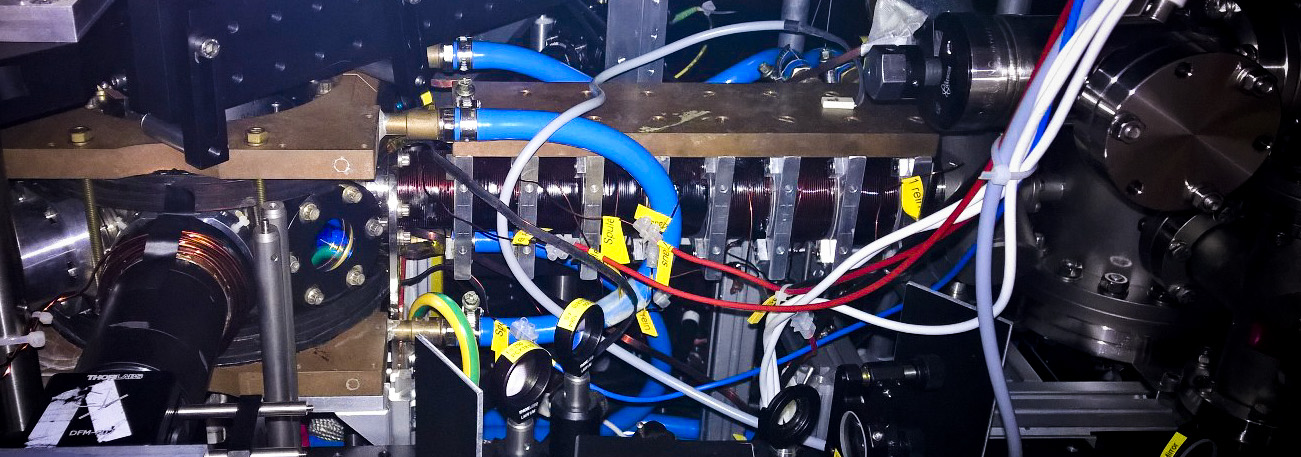
\includegraphics[width=\textwidth]{experiment}
\end{subfigure}
\caption{Photograph of the core-part of the experiment. On the left the octagon-shaped vacuum chamber is visible, with viewports and lenses, focussing beams for the optical dipole trap and the \textsc{mot}. On the right one can see the oven and the Zeeman-slower connecting both parts.}
\label{experiment}
\end{figure}
The key feature of the experiment is the possibility to prepare few atoms in a microscopic dipole trap with high control over their number. A precise description of the experiment is found in \cite{friedhelm}. A briefer summary of this is given in this paragraph.

The experiments are carried out in the so called microtrap, that for the lowest occupied levels can be approximated by a one-dimensional harmonic oscillator. To fill this potential down to the ground state a big reservoid of cold atoms has to be prepared before activating this main stage of the experiment.

After vaporizing Lithium in an oven, the first component of the experiment is the Zeeman slower. When leaving the oven, the atoms are very hot and propagate at velocities, that are too large to trap them in the \textsc{mot} or dipole trap. The Zeeman-slower reduces this speed using radiation pressure while adapting for the the different doppler shifts, exploiting the Zeeman-effect. The slower is essentially a large tube behind the oven shutter surroundet by coils, that provide a different magnetic field value at every point of the apperatus. A strong laserbeam is pointing along the slower. When the beam is in resonance with an atomic transition, the photons get absorbed and the atoms are pushed in the direction of the laser. Because the spontanious emission is directed in random directions, this leads to slowing of the cloud. The atoms however, due to the Doppler-effect see the light blue detuned when flying at high velocities. If the frequency of the laser-beam is adapted to match the resonance frequency for the respective speed, the atoms will be slowed down, but therefore will no longer absorb photons of the same frequency. Therefore different magnetic fields shifts the atomic levels to match the frequncy of the laser everywhere along the legth of the tube and achieve enough cooling to trap the atoms in the \textsc{mot}. 

It consists of six counterpropagating near-resonsant laser-beams. The usage of many retroreflected beams in different directions make it possible to not only force the atoms in a certain direction like in the Zeeman-slower, but to affect all of them with a high absolute speed value and push in the opposite way, in this manner reducing the overall average-speed and therefore cooling the gas. However, because the force of the laserbeams alone is only velocity-dependent, slow particles would exit the center of the crossed beams over time. That is why in a magneto-optical trap a magnetic quadrupole-field is applied, that has zero strength in the middle and will increase when moving further away from the center. The Zeeman-effect shifts the level-distace for the outmoving atoms towards the frequency of the laser, which will then apply a force, dependent on the spatial position, enabeling not only cooling but trapping and compression of the gas-sample. The natural linewith of the used transition limits the cooling of the \textsc{mot} to a temperature of around 140 \mu K. The system used in this experiment can store around 10⁸ atoms. 

The temperature however has to be reduced much further to match the requirements of the experiment later on. The next step on this ladder is the crossed dipole trap. \begin{figure}[h]
\centering
\begin{subfigure}[b]{0.8\textwidth}
                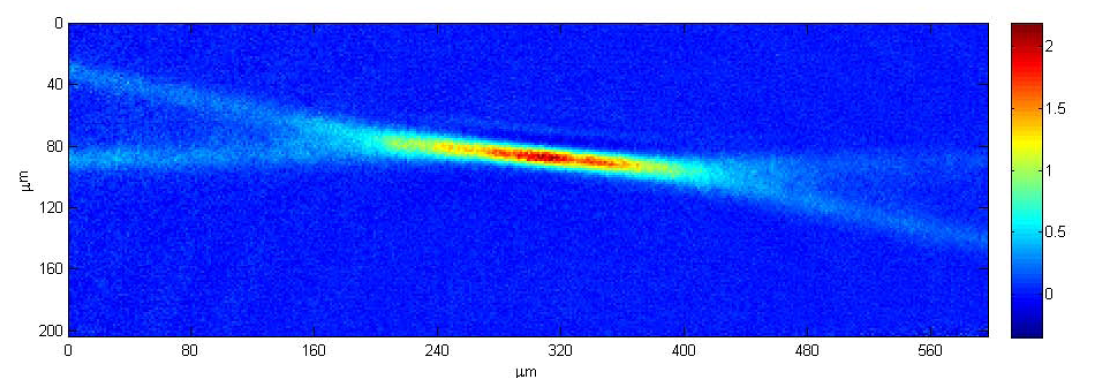
\includegraphics[width=\textwidth]{dipolefoto}
\end{subfigure}
\caption{Absorbtion image of the crossed dipole trap \cite{lompe}.}
\label{experiment}
\end{figure}
It uses the laserbeam of a 200 W Ytterbium fiber-laser (\textsc{ipg ylr-200-lp}) that is far red-detuned from the atomic transitions at 1070 nm. The beams focus lies within the \textsc{mot}, with a waist of approximately 40 \mu m \cite{lompe}. After leaving the vacuum chamber, a mirror system guides it back in at a different angle, forming the crossed trap shape. To trap the most atoms possible the laser is ramped up to full power, leading to a trap depth of over 3 mK. To further cool the sample the power is slowly ramped down, so the hottest atoms escape the potential and the rest of the cloud thermalises at a lower temperature (evaporative cooling). A small, tightly focussed infrared laser-beam at 1064 nm, that intersects the crossed dipole-trap then formes the microtrap (\textsc{mephisto S} from Innolight). The small dimensions of the trap result in high spacing between the allowed harmonic vibrational levels. To control the atom number in the microtrap, a magnetic field gradient tilts the dipole-potential. That leads to the escape of all atoms above a certain level and using this technique one can control the number of atoms between 0 and 10 atoms with high preperation fiddelity. To see the atoms, the microtrap is shut down and the remaining atoms are again trapped in a smaller \textsc{mot}. The resulting flourescence is caught by an objective and projected at the sensor of a \textsc{ccd}-camera. 



\chapter{Theory}

To understand the function of an optical dipole-trap one has to understand how far detuned light, more specificly the electric field component, interacts with a neutral atom. There are several models providing different levels of accuracy for the respective application. The atom can be treated rather classically by regarding it as a harmonic oscillator driven by an electric field. It can be treated semiclassically by considering the quantum nature and structure of the atom while still approximate the incoming light as electromagnetic waves. In this model the problem can be solved in second-order pertubation theory. The third approach is treating the atom quantum mechanically as well as the light, now consisting of quantised photons interacting with the atom. For this thesis only the first two approaches are relevant. 

\section{The Hamiltonian}

The problem of interaction between an atom, laser-light and in the case of this experiment also magnetic fields is represented by different parts in the total hamiltonian. The basis for all calculations is the atomic hamiltonian of the regardet Lithium-atoms $H_A$. The atom-light-interaction is represented by the Hamiltonian of the light itself $H_L$ and the interaction Hamiltonian $H_{AL}$ while the last contribution is the magnetic field Hamiltonian $H_M$.
\begin{equation}
H=H_A+H_L+H_{AL}+H_{M}
\end{equation}\label{hamiltonian}

\section{Lithium Level-structure}
The atomic hamiltonian $H_A$ coresponds to the energy of the atomic species that is used in our experiment, which is Lithium-6. Lithium is a fermionic alkali-metal, whose electronic structure is mostly dependent of its one valence electron \cite{gehm}. In this approximation, the \textit{central-field approximation}, the two other bound electrons on the most inner level only contribute to the central electric field, that is suppost to be sphericaly symetric. Thus the calculation can follow the well understood model of hydrogen. The ansatz in this case is considering an elelctron with the reduced mass $\mu$ in a coulomb-potential.
\begin{equation}
U(\boldsymbol{r})=-\frac{e^2Z}{4\pi\epsilon_0\boldsymbol{r}}
\end{equation}
That leads to the Hamiltonian:
\begin{equation}
H_A=\frac{p^2}{2\mu}-\frac{e^2Z}{4\pi\epsilon_0\boldsymbol{r}}
\end{equation}
Solving the Schrödinger-Equation considering this Hamiltonian leads to a set of wave-functions characterized by the quantum numbers $N,L,m_L$, $N$ being the main quantum number, $L$ the angular momentum quantum number and $m_L$ the projection onto the coordinate axis. The energy-levels for different $L$ are degenerate, but when the spin of the valence electron is considered this degeneracy is broken and the coupling of this spin to the orbital angular momentum leads to the fine-structure picture in which $J=l\pm S$  and $m_J=J,J-1,\dots,-J+1,J$ are the respective quantum numbers.
\begin{figure}[H]
\begin{center}
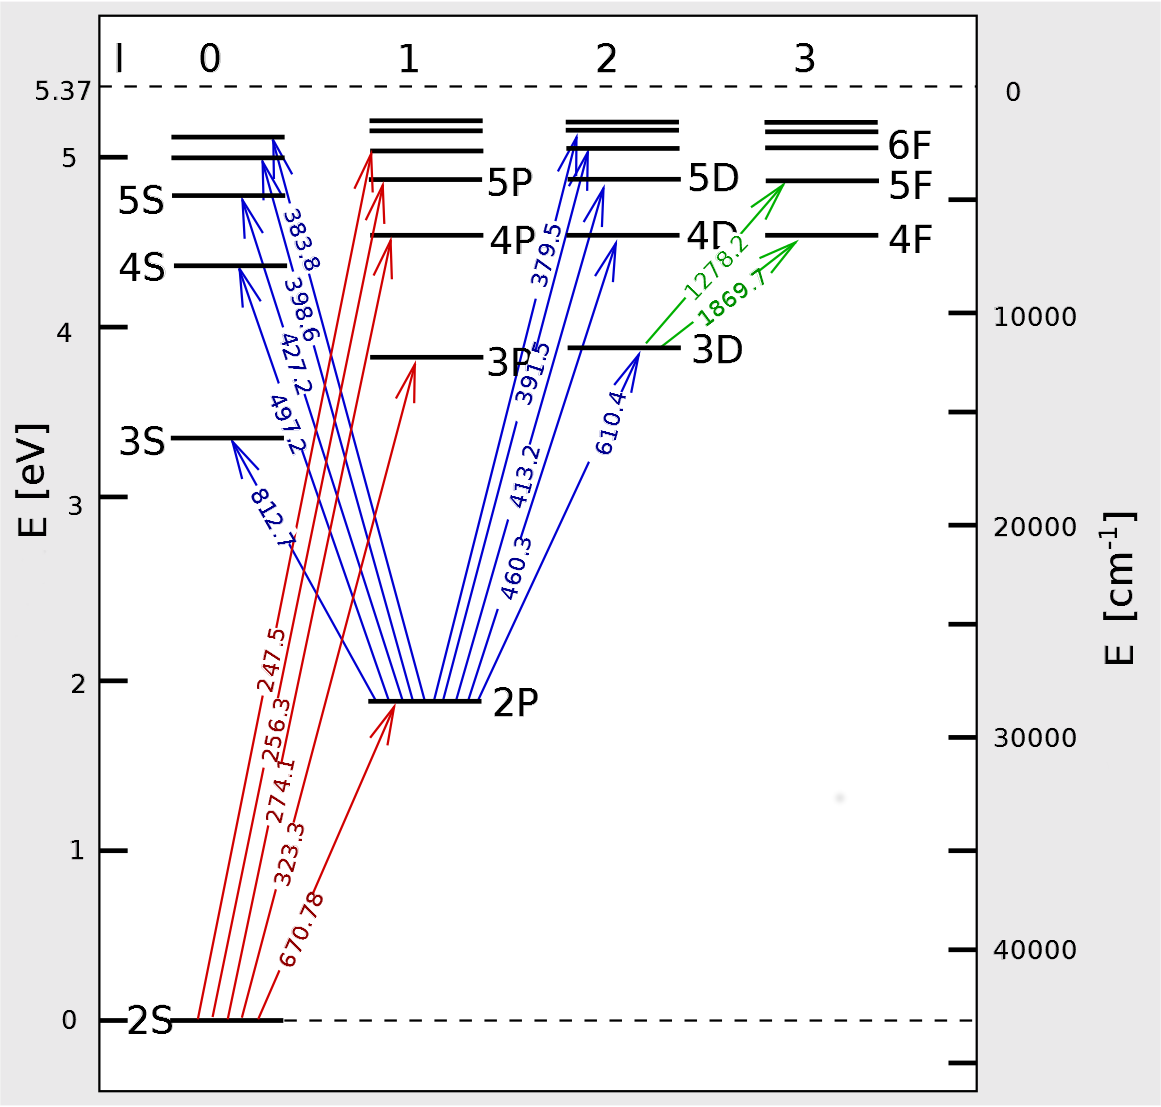
\includegraphics[scale=.4] {levels2}
\end{center}
\caption{Level structure of Lithium with the respective transitions, according to selection rules \cite{transitions}.}
\label{levels2}
\end{figure}
Nevertheless the real Lithium-atom has a substructure arising from interaction of the spin of the core with the angular momentum of the orbit. This effect results in the hyperfinestructure that breaks the degeneracy of the levels with same quantum number $J$. In the picture of hyperfinestructure the total angular momentum and the spin of the core $I$ couple to the new total angular momentum $F=J\pm I$ with their respective projections $m_F=F,F-1,\dots,-F+1,F$ that result in a even finer splitting of the lines, and fully characterize a lithium-atom.

\begin{figure}[H]

\begin{center}
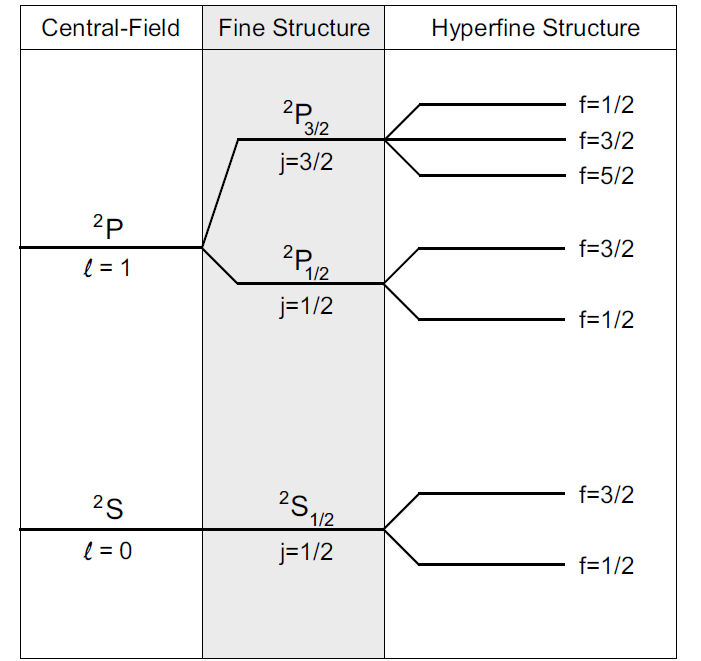
\includegraphics[scale=.5] {levels1}
\end{center}
\caption{Extract of the level structure for Lithium-6 in the fine and hyperfine regime \cite{gehm}}
\label{levels1}
\end{figure}

\section{Magnetic Field}

Within the experiment, the regarded atoms are exposed to strong magnetic fields. Therefore, additionally the Zeeman-Effect moves the respective levels contributing to the \textsc{ac}-Stark-Shift. In this approach we simply regard both effects as independent pertubations to the basic Hamiltonian. At strong magnetic fields, as used in the experiment, the Paschen-Back-Effect for hyperfine states dominates and instead of $F$ and $m_F$, the quantum numbers $J$ and $m_J$ are still “good“. Therefore the formula for the shift of each state is given by:
\begin{equation}
\Delta E=g_Jm_j\hslash\gamma B
\end{equation}
With $\gamma=e/(2m_e)$ and $g_J$ being the Landé-factor. The results are new values of energy-difference i.e. detuning for the respective transitions that now have a different contribution to the \textsc{ac}-Stark-Effect. 

\newpage
\newpage
\section{AC-Stark-Shift}
The \textsc{ac}-Stark-Shift arises from the interaction of electric fields with the regarded atom. Before treating this problem quantum-mechanicaly in terms of our Hamiltonian (\ref{hamiltonian}), we look at the problem in a classical model, that already results in a formula, that is very accurate in certain systems. 
\subsection{Lorentz Oscillator Model}

 Classicaly the problem of light-matter-interaction can be described in terms of an atomic dipole moment induced by an oscillating electric field, following \cite{dipole}. The atom is hereby described as a damped harmonic ocillator driven by the field. Intuitively one can think of the electrons and the core being pulled away from each other by the electric force, resulting in an oscillation against each other. The potential arising from these conditions is the following\footnote{The force on a dipole is given by \cite{factor}:
\begin{equation*}
\boldsymbol{F}=(\boldsymbol{p}\cdot\nabla)\boldsymbol{E}
\end{equation*}
We know that the following holds:
\begin{equation*}
\nabla(\boldsymbol{p}\cdot\boldsymbol{E})=\boldsymbol{p}\times(\nabla\times\boldsymbol{E})+\boldsymbol{E}\times(\nabla\times\boldsymbol{p})+(\boldsymbol{p}\cdot\nabla)\boldsymbol{E}+(\boldsymbol{E}\cdot\nabla)\boldsymbol{p}
\label{dipoleforce}\end{equation*}
We consider the trap to consist of a retro-reflected laserbeam, that is in phase, so the B-field-component of the electromagnetic wave is onsidered to be 0 as well as $\nabla\times\boldsymbol{E}=-\partial\boldsymbol{B}/\partial t=0$. In our case the dipole-moment is not constant but \(\boldsymbol{p}=\alpha \boldsymbol{E}\) and thus becomes:
\begin{equation*}
\nabla(\boldsymbol{p}\cdot\boldsymbol{E})=\alpha\boldsymbol{E}\times(\nabla\times\boldsymbol{E})+\alpha\boldsymbol{E}\times(\nabla\times\boldsymbol{E})+(\alpha\boldsymbol{E}\cdot\nabla)\boldsymbol{E}+\alpha(\boldsymbol{E}\cdot\nabla)\boldsymbol{E}
\end{equation*}
which becomes:
\begin{align*}
\nabla(\boldsymbol{p}\cdot\boldsymbol{E})&=2\alpha(\boldsymbol{E}\cdot\nabla)\boldsymbol{E}=2(\boldsymbol{p}\cdot\nabla)\boldsymbol{E}\\
\Rightarrow \boldsymbol{F}&=\frac{1}{2}\nabla(\boldsymbol{p}\cdot\boldsymbol{E})
\end{align*}
To get the corresponting potential one has to integrate the force. For a rapidly oscillating field we futher have to take the time average to get an effective value for the trapping potential.
\begin{equation*}
U=-\frac{1}{2}\mean{\boldsymbol{p E}}
\end{equation*}}:
\begin{equation}
U=-\frac{1}{2}\mean{\boldsymbol{p E}}
\label{dipole}
\end{equation} 
Here $\boldsymbol{p}$ is the induced dipole moment, $\boldsymbol{E}$ the electric field. The time-average is introduced since the electric field in an electro-magnetic wave is oscillating very fast and the atom “feels“ an effective potential averaged over the oscillation. If we only consider the real part of $\boldsymbol{p}\boldsymbol{E}\propto \cos^2$, the time average is $\mean{\boldsymbol{p}\boldsymbol{E}}=1/2 \mathrm{ Re}(\alpha)E^2$. One can rewrite (\ref{dipole}) in terms of the Intentity $I=1/2\epsilon_0cE^2 $:
\begin{equation}
U=-\frac{1}{2\epsilon_0 c}\mathrm{Re}(\alpha)I
\end{equation} 

To calculate the exact potential one has to obtain a value for $\alpha$. In this classical description an electron is considered bound to the core elastically with the oscillation eigenfrequency $\omega_0$ corresponding to the optical transition frequency. In our practical case that is the frequency of the Lithium-D2-Line. In a real atom, there are of course multiple resonances, corresponding to multible states of the electron, thus this is approximation yields only for certain cases in which the system can also be regarded as a quantummechanical two-state-system. We will later see, that while this approach leads to a very accurate calculation for the Lithium ground state, it can not at all be applied to the calculation of the trapping potential for the first excited state, since there exists no single dominant transition, but multiple resonances, all contributing to the respective energy-shift, in contrast to the groundstate.

The polarizability now can be calculated by solving the equation of motion of a driven and damped harmonic oscillator.
\begin{equation}
\ddot x+\Gamma_\omega\dot x+\omega^2_0x=-\frac{eE(t)}{m_e}
\end{equation} 
for that the solution can be calculated using basic tools for differential-equation-solving. The result is then:
\begin{equation}
\alpha=\frac{e^2}{m_e}\frac{1}{\omega^2_0-\omega^2-\mathrm{i}\omega\Gamma_\omega}
\end{equation} 
With
\begin{equation}
\Gamma_\omega=\frac{e^2\om^2}{6\pi\epsilon_0m_ec^3}
\end{equation}
We can substitute $e^2/m_e=6\pi\epsilon_0c^3\Gamma_\omega/\om^2$ and define the on-resonance damping rate $\Gamma:=(\om_0/\om)^2\Gamma_\omega$ witch results in the form:
\begin{equation}
\alpha=6\pi\epsilon_0c^3\frac{\Gamma/\om^2_0}{\omega^2_0-\omega^2-\mathrm{i}(\om^3/\om^2_0)\Gamma}
\end{equation} 
We now can plug the real part of this expression in (\ref{dipole}) and obtain the very known formula:
\begin{equation}
U_{dip}(\boldsymbol{r})=-\frac{3\pi c^2}{2\om^3_0}(\frac{\Gamma}{\om_0-\om}+\frac{\Gamma}{\om_0+\om})I(\boldsymbol{r})
\label{classic}\end{equation}
In this case, the damping parameter $\Gamma$ corresponds to the linewidth of the optical transition, which numerical value is $\Gamma=5.8724 \unit{MHz}$ for the considered D2-Line \cite{gehm}.

\subsection{Energy-Shift in Pertubation Theory}

After this classical treatment, we come back to calculating the same effect quantum-mechanically. For calculating the energy-shift for the first excited state, this is the only way to get a trustworthy result since in contrast to the ground state of Lithium it can not be approximated by a two-level-system with only one transition. Therefore we have to solve the problem more precicely. 

The interaction of the atom with laser-light is described by the two additional parts in the original hamiltonian (\ref{hamiltonian}) $H_L+H_{AL}$. The light-hamiltonian $H_L$ is hereby negligible, because the regarded laser-light of the used dipole-trap is farly detuned from the relevant transition resonances. Therefore the only relevant part of this set of terms is the interaction-hamiltonian, which depends on the dipole-operator $\mu$ and the electric-field-operator $E$ and has the following form: $H_{AL}=-\mu E=-e\boldsymbol{r} E$. It can be treated as a small pertubation of the atomic hamiltonian, thus in the relevant second-order pertubation-theory the energy-shift is the following \cite{dipole}:
\begin{equation}
\Delta W=\sum_{k\neq j}\frac{|\braopket{j}{H_{AL}}{k}|^2}{W_k-W_j}
\label{pertub1}
\end{equation}
Although the hyperfine splitting is highly relevant for the experiment itself, it is sufficient for the calculation of the Stark-Shift to only consider the fine-structure regime. Aspecially at high-strength magnetic fields, the hyperfine Paschen-Back-Effect leads to degeneracy of the different hyperfine states and the total angular momentum $J$ is a "good quantum-number" again. In the low-field-regime the corrections due to hyperfine-splitting are small, because of the little energy-differences compared to the relevant transitions between the levels in the fine-structure-regime and the considered large detuning of the dipole-trap-light. Hence also there this picture is sufficient. In this case (\ref{pertub1}) can be expressed in terms of $J$ and $m_J$ and with the explicit form of $H_{AL}$ this becomes\cite{alpha}:
\begin{equation}
\Delta W_{Jm_j}=-e^2\sum_{K\neq J}\sum_{m_k}\frac{\braopket{Jm_J}{\boldsymbol{r}E}{Km_K}\braopket{Km_K}{\boldsymbol{r}E}{Jm_J}}{W_k-W_j}\boldsymbol{r}E\label{pertub2}
\end{equation}
The main problem now is to calculate the coupling of different angular momenta. That is why most of the calculation is dedicated to simplify the calculation of all relevant Clebsch-Gordan coefficients.\\\\
We will now describe the electric field in terms of irreducible tensor operators:
\begin{align}
E_{\pm}=\mp\frac{1}{2}\sqrt{2}(E_x\pm \mathrm{i}E_y),\ \ \ E_0=E_z\\
r_{\pm}=\mp\frac{1}{2}\sqrt{2}(r_x\pm \mathrm{i}r_y),\ \ \ r_0=r_z\\
\end{align}
In this notation we can rewrite (\ref{pertub2}) in terms of these operators:
\begin{equation}
\Delta W_{Jm_j}=-e^2\sum_{K\neq J}\sum_{m_k}\sum_{\mu\nu}(-1)^{\mu+\nu}E_\mu E_\nu\frac{\braopket{Jm_J}{r_{-\mu}}{Km_K}\braopket{Km_K}{r_{-\nu}}{Jm_J}}{W_k-W_j}\label{pertub3}
\end{equation}
With $\mu=0,\pm1$. Now, we define the following sum, that will be used later on. Note that is a simple shorting for simplification.
\begin{equation}
\mathcal{E}(L,m_L):=\\sum_{\mu\nu}\sqrt{2L+1}(-1)^{m_L}\threej{1}{1}{L}{\mu}{\nu}{-m_L}E_\mu E_\nu\label{irreducible}
\end{equation}
We here also use the Wigner 3-j-symbol-notation\footnote{The Wigner 3-j symbol and 6-j symbol are definded in terms of Clebsch-Gordan-Coefficients:\begin{align}\threej{j_1}{j_2}{j_3}{m_1}{m_2}{m_3}:=&\frac{(-1)^{j_1-j_2-m_3}}{\sqrt{2j_3+1}}\braket{j_1m_1j_2m_2}{j_3-m_3}\\\sixj{j_1}{j_2}{j_3}{j_4}{j_5}{j_6}:=&\sum^6_{m_j}(-1)^{\sum^6_{k=1}(j_k-m_k)}\threej{j_1}{j_2}{j_3}{m_1}{m_2}{-m_3}\threej{j_1}{j_5}{j_6}{-m_1}{m_5}{m_6}\\\times&\threej{j_4}{j_5}{j_3}{m_4}{-m_5}{m_3}\threej{j_4}{j_2}{j_6}{-m_4}{-m_2}{-m_6}\label{jsymbols}\end{align}}. Therefore we can write the product in (\ref{pertub3}) in terms of this sum: 
\begin{equation}
E_\mu E_\nu=\sum^2_{L=0}\sum^L_{m_L=-L}\sqrt{2L+1}(-1)^{m_L}\threej{1}{1}{L}{\mu}{\nu}{-m_L}\mathcal{E}(L,m_L)
\end{equation}
For later-on simplification, we can calculate (\ref{irreducible}) explicitly for different combinations of $L$ and $m_L$.
\begin{align*}
\mathcal{E}(0,0)&=-\frac{1}{\sqrt{3}}(E^2_0-2E_{-1}E_{1})=-\frac{1}{\sqrt{3}}(E^2_z-2(-\frac{1}{2}(E_x+\mathrm{i}E_y)(E_x+\mathrm{i}E_y))\\&=-\frac{1}{\sqrt{3}}(E^2_z+E²_x+E^2_y)=-\frac{1}{\sqrt{3}}E^2\\
\mathcal{E}(1,\pm 1)&=0\\
\mathcal{E}(1,0)&=0\\
\mathcal{E}(2,\pm2)&=E^2_{\pm1}=\frac{1}{2}(E_x\pm \mathrm{i}E_y)^2\\
\mathcal{E}(2,\pm1)&=(E_x\pm \mathrm{i}E_y)E_z\\
\mathcal{E}(2,0)&=\sqrt{\frac{2}{3}}(E^2_0+E_{-1}E_1)=\sqrt{\frac{2}{3}}(E^2_z+\frac{1}{2}E^2_z-\frac{1}{2}E^2_z-\frac{1}{2}(E^2_x+E^2_y))\\&=\frac{1}{\sqrt{6}}(3E^2_z-E^2)
\end{align*}
After finishing that horrible calculation, the next step is to evaluate the sum in (\ref{pertub3}), which is even more terrifying, as you can imagine!

The first step is to evaluate the inner part, that is the summation over the respective magnetic quantum numbers $m_J$. Thus we give it an own name and define:
\begin{equation}
\mathcal{S}(J,m_J)=\sum_{m_k}\sum_{\mu\nu}(-1)^{\mu+\nu}E_\mu E_\nu\braopket{Jm_J}{r_{-\mu}}{Km_K}\braopket{Km_K}{r_{-\nu}}{Jm_J}\label{sum}
\end{equation}
The matrix elements can be calculated using the Wigner-Eckart theorem\footnote{The Wigner-Eckart theorem simplifies the calculation of matrix-elements in a spherical basis and breaks it down to the calculation of few reduced matrix elements. For an irreducible tensor-operator $T^r_q$ between two angular-momentum eigen-states the following holds \cite[17]{wigner}:
\begin{equation}
\braopket{j,m_j}{T^r_q}{k,m_k}=\braopket{j}{|T^r|}{k}C^{jm_j}_{rqkm_k}
\end{equation}
In this formula $r$ denotes the rank of the tensor, and $q$ is simply the respective component of the tensor. Writing this in terms of the 3-j symbols yields:
\begin{equation}
\braopket{j,m_j}{T^r_q}{k,m_k}=(-1)^{j-m_j}\threej{j}{r}{k}{-m_j}{q}{m_k}\braopket{j}{|T^r|}{k}
\end{equation}
The resulting reduced matrix elements are independent of the respective component of the operator and the $m$-quantum-number. Therefore for every pair of angular-momentum quantum numbers $j$ and $k$ only one reduced matrix element has to be calculated to evaluate all elements of eigenstates involving said angular momenta.}.
\begin{align}
\mathcal{S}(J,m_J)=&(-1)^{J-K}|\braopket{J}{|r|}{K}|^2\times\notag\\&\sum_L\sqrt{2L+1}\sum_{m_L}\mathcal{E}(L,m_L)\sum_{\mu\nu}(-1)^{\mu+\nu}(-1)^{m_L}\threej{1}{1}{L}{\mu}{\nu}{-m_L}\times\notag\\&\sum_{m_K}\left[(-1)^{J-m_J}\threej{J}{1}{K}{-m_J}{-\mu}{m_K}(-1)^{K-m_K}\threej{K}{1}{J}{-m_K}{-\nu}{m_J}\right]\label{sum2}
\end{align}
Note, that the first part of this term can be written in this way because because using the Wigner-Eckert theorem the tensor operator in the matrix element now has become the normal spherical coordinate-operator in the respective reduced matrix element, which of course is hermitian. The sum over $\mu,\nu$ and $m_K$ can be evaluated and rewritten in terms of the 6-j symbol.
\begin{align}
&\sum_{\mu\nu}(-1)^{\mu+\nu}(-1)^{m_L}\threej{1}{1}{L}{\mu}{\nu}{-m_L}\times\notag\\&\sum_{m_K}\left[(-1)^{J-m_J}\threej{J}{1}{K}{-m_J}{-\mu}{m_K}(-1)^{K-m_K}\threej{K}{1}{J}{-m_K}{-\nu}{m_J}\right]\notag\\&\ \ =(-1)^{2J}(-1)^{J-m_J}\threej{J}{L}{J}{-m_J}{0}{m_J}\sixj{J}{1}{K}{1}{K}{L}\delta_{m_L,0}
\end{align}
This, together with the values for $\mathcal{E}(L,m_L)$, leads to the fact, that only terms with $L=0,2$ and $m_L=0$ remain and the following holds:
\begin{align}
\mathcal{S}(J,m_J)=&(-1)^{J-K}|\braopket{J}{|r|}{K}|^2\times\notag\\&\sum_{L}\mathcal{E}(L,0)\sqrt{2L+1} (-1)^{J-m_J}\threej{J}{L}{J}{-m_J}{0}{m_J}\sixj{J}{1}{K}{1}{K}{L}\label{sum3}
\end{align}
Now, we arrive at the point, where we can go back to evaluating (\ref{pertub2}). The finding in (\ref{sum3}) means, that we can decompose $\Delta W_{Jm_J}$ into a sum over different $L$:
\begin{equation}
\Delta W_{Jm_J}=\sum_L\Delta W^L_{Jm_J}
\end{equation}
in which each of the components can be written, using the form of (\ref{sum3}).
\begin{align}
\Delta W^L_{Jm_J}=&-e^2\sum_{K\neq J}\frac{\braopket{J}{|r|}{K}|^2}{W_K-W_J}\mathcal{E}(L,0)\sqrt{2L+1}\notag\\&(-1)^{J+K} (-1)^{J-m_J}\threej{J}{L}{J}{-m_J}{0}{m_J}\sixj{J}{1}{K}{1}{K}{L}\label{pertub4}
\end{align}
For this equation we can analyse the only two different cases, namely for $L=0,2$. If we evaluate both components and use the values vor $\mathcal{E}(1,0)$ and $\mathcal{E}(1,0)$, we get to the both contributions to the energy-shift:
\begin{align}
\Delta W^0_{Jm_J}=&-e^2E^2\frac{1}{3(2J+1)}\sum_{K\neq J}\frac{\braopket{J}{|r|}{K}|^2}{W_K-W_J}\\
\Delta W^2_{Jm_J}=&-e^2(3E^2_z-E^2)\sqrt{\frac{5J(2J-1)}{6(2J+3)(J+1)(2J+1)}}\ \times\notag\\
&\frac{3m^2_J-J(J+1)}{J(2J-1)}\sum_{K\neq J}(-1)^{J+K}\sixj{J}{1}{K}{1}{J}{2}\frac{\braopket{J}{|r|}{K}|^2}{W_K-W_J}
\end{align}
We now chose the electric field to be directed along the z-axis: $\boldsymbol{E}=E\hat{\boldsymbol{z}}$ so we can say, that $E^2_z=E^2$. Thus follows:
\begin{align}
\Delta W^2_{Jm_J}=&-\frac{1}{2}e^2E^24C\ \times\notag\\
&\frac{3m^2_J-J(J+1)}{J(2J-1)}\sum_{K\neq J}(-1)^{J+K}\sixj{J}{1}{K}{1}{J}{2}\frac{\braopket{J}{|r|}{K}|^2}{W_K-W_J}\label{alpha21}
\end{align}
We are hereby shortening $C:=\sqrt{5J(2J-1)/6(2J+3)(J+1)(2J+1)}$.
Note, that if the z-direction also defines the quantisation axis in a magnetic field, this means assuming $\pi$-polarized laser-light. If the light is then supposed to be $\sigma$-polarized, the z-component has to be considered individually and is holds $E^2_z=1/2\ E^2$.
We now draw an analogy to the classical calculation and link the total energy-shift to the dipole potential by defining a polarizability, composed of the now defined scalar and tensor polarizability.
\begin{align}
\alpha:=&e^2\left[\alpha^0_J+\frac{3m^2_J-J(J+1)}{J(2J-1)}\alpha^2_J\right]\\
\notag\\
\alpha^0_J=&\frac{2}{3(2J+1)}\sum_{K\neq J}\frac{|\braopket{J}{|r|}{K}|^2}{W_K-W_J}\\
\alpha^2_J=&4C\sum_{K\neq J}(-1)^{J+K}\sixj{J}{1}{K}{1}{J}{2}\frac{|\braopket{J}{|r|}{K}|^2}{W_K-W_J}
\end{align}
An additional factor has to be multiplied in analogy to the classical formula. The electric field is oscillating and the average thus results in a factor of $1/2$, because we did not take the time into account, when calculating the polarizability.
\begin{align}
U=&-\frac{1}{2}\alpha E^2\notag\\
U=&-\frac{1}{4}e^2\left[\alpha^0_J+\frac{2m^2_J-J(J+1)}{J(2J-1)}\alpha^2_J\right]E^2\label{shift}
\end{align}

\section{Dipole Traps}

The \textsc{ac}-Stark-Shift, as described above can, as stated in the beginning, be used to trap neutral atoms. We so far have seen, that an electric field induces a dipole moment in the atom that leads to a dipole-potential.The resulting force is proportional to the gradient of the intensity-distribution around the atom, therefore to understand how a dipole trap works exactly, one has to study the properties of the applied beams. Lasers normally emmit gaussian beams. The intensitiy distribution along the radial profile at a given point on the course of the beam is \cite{dipole}:
\begin{equation}
I(r)=\frac{2P}{\pi w^2}\mathrm{exp}(-2\frac{r^2}{w^2})
\end{equation}
With $r$ being the radal coordinate, $P$ the power of the beam and $w$ the waist. In contrast to simle ray-optics, the focus of the gaussian beam is not point like but has a finite waist $w_0$. At this point the intensity of the focussed laser-beam is at its maximum:
\begin{equation}
I_{\mathrm{max}}=\frac{2P}{\pi w^2_0}
\end{equation}
This determines the deepest point in the potential, indepedent of the exact geometry of the trap, in case the center has a gaussian form. This is the case for both dipole-traps used in the experiment, that are described in the previous section.
\chapter{Calculation of the AC-Stark-Shift}

The calculation of the \textsc{ac}-Stark-Shift is done, using the formulas resulting from pertubation theory, as carried out in the previous sections. The first part of this chapter reviews the main results regarding the polarizabilities of the ground and first excited state. This will reveal also whether the excited state can also be trapped in the high intensity region of the lasers and how the trapping compares to that of the ground state. All calculations use the computer algebra system mathematica.\\For the meassurement, testing the theoretical foundation, that is presented in this thesis, concrete shift calculations are made regarding the big, crossed dipole trap. At the end of this section, values for the small microtrap will be presented, that will suggest, in how far the goal of imaging atoms in small traps and single sites of optical lattices can be managed. The magnetic field, and thus the quantisation axis is definde to be along the z-direction.

\section{Polarizability}
For the calculation of the polarizabilities for the respective states, the geometry and power of the used laser-beams are not important, since it only depends on the wavelength of the incoming light and on its polarization, that has a notable role for the tensor-polarizability in the vicinity of a transition resonance and renders unimportant, when using very far detuned trap-light. Before talking about concrete results, we recall the formulas given in the theory-section. 
\begin{align}
\alpha=&\left[\alpha^0_J+\frac{3m^2_J-J(J+1)}{J(2J-1)}\alpha^2_J\right]\\
\notag\\
\alpha^0_J=&\frac{2}{3(2J+1)}\sum_{K\neq J}\frac{|\braopket{J}{|r|}{K}|^2}{W_K-W_J}\notag\\
\alpha^2_J=&4C\sum_{K\neq J}(-1)^{J+K}\sixj{J}{1}{K}{1}{J}{2}\frac{|\braopket{J}{|r|}{K}|^2}{W_K-W_J}\notag
\end{align}
Following \cite{magic01}, the polarizability is calculated using atomic units (a.u.). For the calculation transitions up to $n=7$ were considered. The respective dipole-transition matrix elements are listed below, together with the energy-differences between the levels.

\begin{figure}[H]
\begin{center}
\begin{tabular}{ccc}
Transition&Matrix-element [$\unit{a.u.}$]&Resonance [$\unit{nm}$]\\\hline\hline\\
$2s_{1/2}-2p_{1/2}$&3.3169&670.791\\
$2s_{1/2}-2p_{3/2}$&4.6909&670.776\\
$2s_{1/2}-3p_{1/2}$&0.183&323.2657\\
$2s_{1/2}-3p_{3/2}$&0.259&323.2657\\
$2s_{1/2}-4p_{1/2}$&0.160&274.1203\\
$2s_{1/2}-4p_{3/2}$&0.226&274.1203\\
$2s_{1/2}-5p_{1/2}$&0.1198&256.2312\\
$2s_{1/2}-5p_{3/2}$&0.169&256.2312\\
$2s_{1/2}-6p_{1/2}$&0.0925&247.5061\\
$2s_{1/2}-6p_{3/2}$&0.131&247.5061\\
$2s_{1/2}-7p_{1/2}$&0.0737&242.5426\\
$2s_{1/2}-7p_{3/2}$&0.1042&242.5426\\
$2p_{3/2}-3s_{1/2}$&3.4403&812.645\\
$2p_{3/2}-4s_{1/2}$&0.9167&497.175\\
$2p_{3/2}-5s_{1/2}$&0.4929&427.313\\
$2p_{3/2}-6s_{1/2}$&0.3268&398.554\\
$2p_{3/2}-7s_{1/2}$&0.2397&383.564\\
$2p_{3/2}-3d_{3/2}$&2.2658&610.366\\
$2p_{3/2}-3d_{5/2}$&6.7975&670.776\\
$2p_{3/2}-4d_{3/2}$&0.8627&460.283\\
$2p_{3/2}-4d_{5/2}$&2.5882&460.289\\
$2p_{3/2}-5d_{3/2}$&0.5015&413.262\\
$2p_{3/2}-5d_{5/2}$&1.5045&413.262\\
$2p_{3/2}-6d_{3/2}$&0.3435&391.535\\
$2p_{3/2}-6d_{5/2}$&1.0306&391.535\\
$2p_{3/2}-7d_{3/2}$&0.2565&379.507\\
$2p_{3/2}-7d_{5/2}$&0.7696&379.507\\\\\hline
\end{tabular}
\end{center}
\caption{Reduced Dipole-Transition-Matrix-Elements \cite{magic01} in a.u. and the respective detuning \cite{NIST_ASD}, i.e. the resonance-energy for the relevant levels: $1s_22s_{1/2}$ and $1s_22p_{3/2}$}
\label{matrixelements}
\end{figure}
Figure \ref{alphages} shows how the polarizability behaves for different levels and different wavelength of the incoming laser-light. In this case, $\pi$-polarized light is assumed. The qualitative behaviour does not change due to different polarizations, only the magnitute of the tensor polarizability. The differences in the practical case of our experiment will be discussed later on.
\begin{figure}[H]
\centering
\begin{subfigure}[b]{0.4\textwidth}
                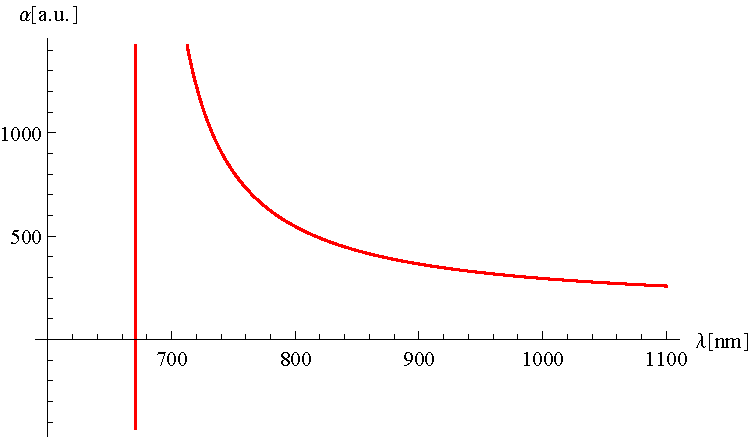
\includegraphics[width=\textwidth]{alphaground}
                \caption{$1s2s_{1/2}$}
\end{subfigure}
\begin{subfigure}[b]{0.4\textwidth}
               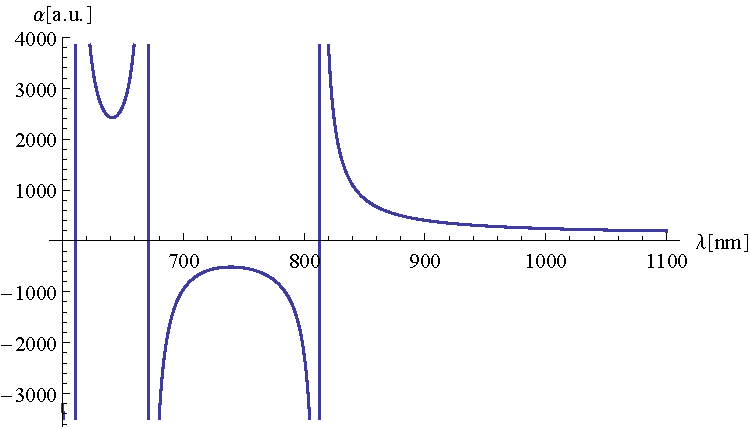
\includegraphics[width=\textwidth]{alphaexited12}
                \caption{$1s2p_{3/2}, |m_j|=1/2$}
\end{subfigure}
\begin{subfigure}[b]{0.4\textwidth}
               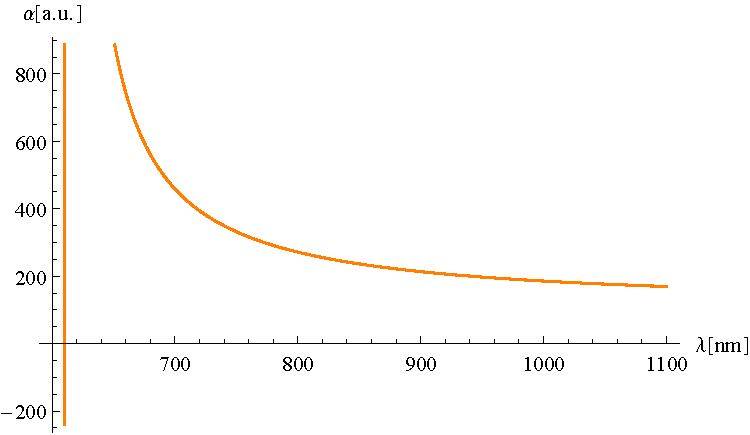
\includegraphics[width=\textwidth]{alphaexited32}
                \caption{$1s2p_{3/2}, |m_j|=3/2$}
\end{subfigure}
\begin{subfigure}[b]{0.4\textwidth}
                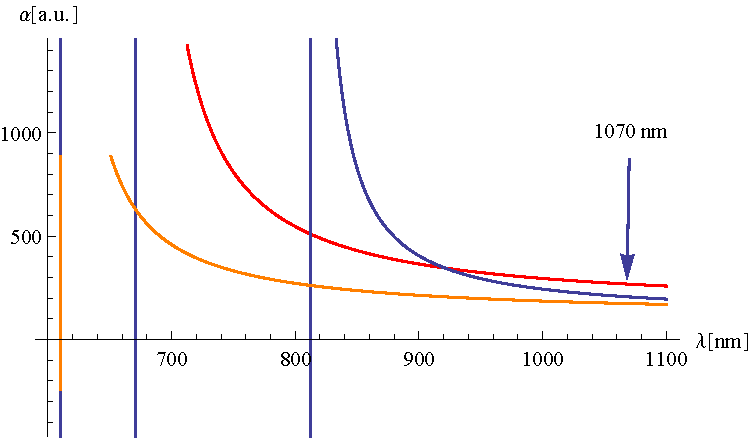
\includegraphics[width=\textwidth]{alphaalltogether}
                \caption{Comparison}
\end{subfigure}




\caption{Polarizability \alpha for the states $1s2s_{1/2}$ (red) , $1s2p_{3/2}, |m_j|=1/2$ (blue) and  $1s2p_{3/2}, |m_j|=3/2$ (orange)}
\label{alphages}
\end{figure}
What can be seen in the plots are some interesting properties. The first important result is, that, considering a far detuned light-source, the ground state, as well as the excited state show positive polarizabilities. This fundamentally contradicts the picture of a two-level system, for example described in \cite{cohen}. In this model, the excited state will be shifted in opposition to the ground state, i.e. the relative sign in the polarizability flips. This reflects the fact, that in a real atom, aspecially in the exited states of Lithium, the structure is much more complicated, than what results from the two-level approximation, because many different levels are roughly in the same energy-range and no single transtion dominates. Practically this results in the fact, that both the ground-state and the first excited states can be trapped in the same type of dipole-trap, because the positive polarizability results in a negative potential. Therefore the atoms are attracted to the highest intensity of the laser-beam. The difference lies in the exact values. For farly detuned light, i.e. above around 1000 nm of wavelength, the ground state shows a higher polarizability, than both excited states, which means, that the potential is deeper for the ground state. From figure \label{relativealpha} can be seen, how the different excited states behave relative to the ground state for the both relevant laser-wavelength for the big and the small dipole-trap in the experiment. As one could expect the difference in the regime of farly detuned light is negligible. As stated in the theory-section, the magnetic field shifts the different levels, depending on their respective angular momentum and magnetic quantum numbers. This results in different values for the detuning, that determines the polarizability. However, at 527 G, that is a high field in the framework of the experiment, the shifts due to the Zeeman-effect are very small and the overall change in the resonance is orders of magnitude below the error in predicting the differential light shift alltogether. This is an important result, thus it tells us, that in cold atom experiments, where different values of magnetic field from weak to strong are used to tune the respective interaction strength, the trapping efficiency is nearly independent from such tunings.

\begin{figure}[h]
\begin{center}
\begin{tabular}{ccc}
State&$\alpha$ at $1070\unit{nm}$ [$\unit{\alpha_{ground}}$]&$\alpha$ at $1064\unit{nm}$ [$\unit{\alpha_{ground}}$]\\\hline\hline\\
$2p_{3/2}, |m_j|=1/2$&0.7694&0.7726\\
$2p_{3/2}, |m_j|=3/2$&0.6487&0.6472\\
\\\hline
\end{tabular}
\end{center}
\caption{Polarizabilities of the excited states for the relevant laser-wavelengths, in relation to the ground state polarizability.}
\label{relativealpha}
\end{figure}

The picture looks different, when cosidering higher frequencies. There, the picture looks different, aspecially when comparing the two excited states with different magnetic quantum number. Below around 900 nm and $m_j=3/2$ the absolute value of the polarizability is much higher than for both other states. Mathematically this can easiest be seen, when looking at the formula for the total polarizability. The tensor-part of this formula is multiplied by a factor, that is -1 or +1, depending on whether $|m_j|=1/2$ or $|m_j|=3/2$. This means, that it decides whether the tensor part is added or subtracted, when calculating the total value. If it is substracted, in case of $|m_j|=3/2$, in the vicinity of many resonances, the diverging terms will cancel each other out and instead of a singularity a finite value is the result.

This does not mean, that one state can be trapped easier. When using laser-light, that is not far detuned from the respective resonances absorbtion effects cause the light to transfer momentum onto the atoms, that thus will heat up and the overall force field is no longer conervative. However using this effects in special settings can also result in effectve trapping and cooling techniques. An optical molasse for example uses a standing wave of circular polarized laser-beams, so that the electric field and thus the polarizability and the respective light-shift are spacially dependent. Using the fact, that for different $m_J$-levels the light shift is different, one can tune the different beams such that after an absorbtion cycle the atoms decay into lower $m_J$-states and thus lose energy and cool down. In an optical dipole trap however, absorbtion is an unwanted heating-effect and therefore it is most efficient, when using laser-light farly detuned from the resonances. In this regime, all magnetic sublevels strive towards the same vale of polarizability, only depending on the scalar part, that is isotropic and does not depend on the light-polarization.

\subsection{Convergence for the calculation}

\begin{figure}[H]
\centering
\begin{subfigure}[b]{0.4\textwidth}
                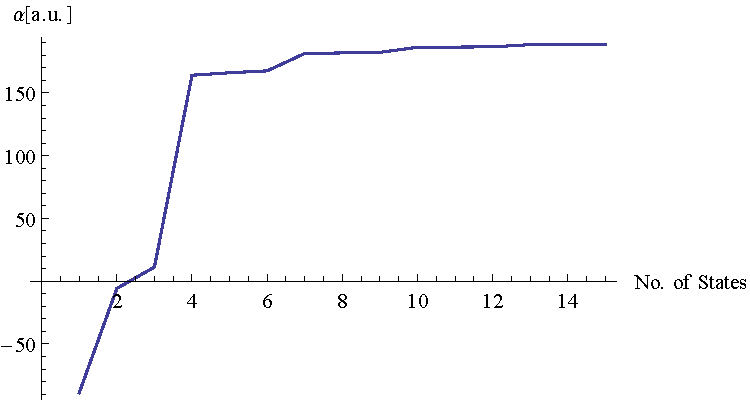
\includegraphics[width=\textwidth]{alphascalarconvexcited}
                \caption{Scalar polarizability $\alpha^0_J$}
\end{subfigure}
\begin{subfigure}[b]{0.4\textwidth}
               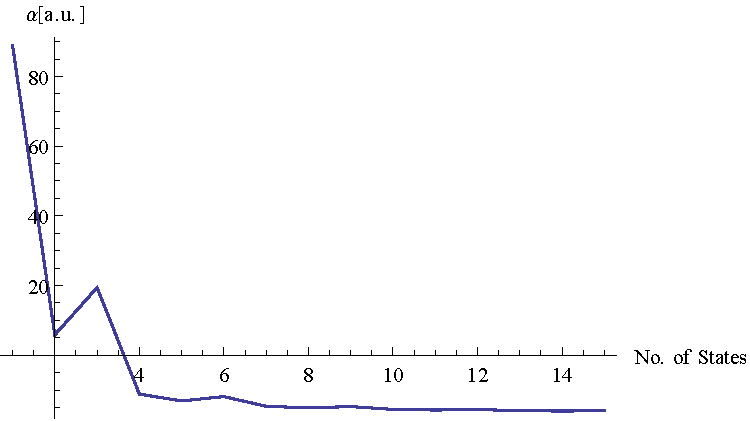
\includegraphics[width=\textwidth]{alphatensorconvexcited}
                \caption{Tensor polarizability $\alpha^2_J$}
\end{subfigure}


\caption{Convergence of the polarizability value for the excited state $1s2p_{3/2}, |m_j|=3/2$ at 1070 nm.}
\label{alphaconv}
\end{figure}

Another interesing question is, how far one has to go in calculating the energy shift in this pertubation framework to get a good approximation of the actual value. The maximum accuracy, as written above, was considering levels up to $n=7$. Figure (\ref{alphaconv}) shows how the value of $\alpha$ changes when considering higher levels. The x-coordinate is simply the index of the states, counted from low to high detuning. One can see, that for the excitet state, when going above $n=3$(Index > 4) the curve seems to converge. However for up to $n=3$, the value of $\alpha$ reaches only 85\% of its value at the full calculation. It reaches 95\% not until considering levels up to $n=5$. This is because all levels further above show little differences in detuning and also in te respective reduced matrix elements and therefore the states contribute similarily to the final result. In the case of the ground state, considering only the two lowest transitions already results in a value that has 99.8\% of the final value. Therefore the high precision calculation when taking into accound higher levels brings little benefit.

\begin{figure}[h]
\centering
\begin{subfigure}[b]{0.4\textwidth}
                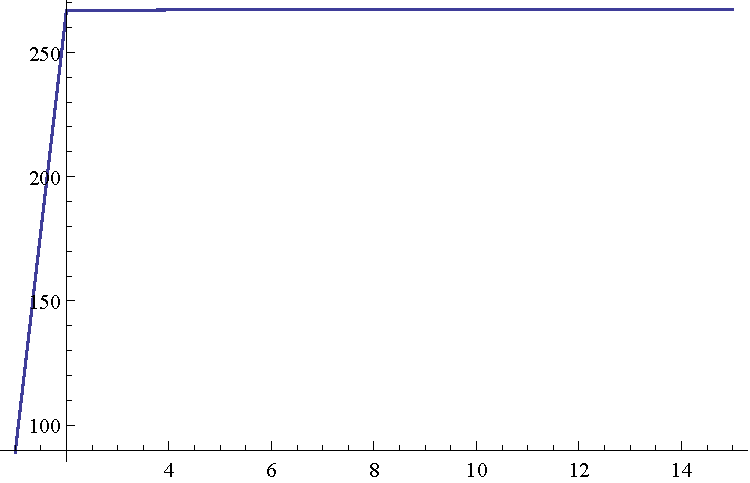
\includegraphics[width=\textwidth]{alphascalarconvground1}
                \caption{Polrizability \alpha}
\end{subfigure}
\begin{subfigure}[b]{0.4\textwidth}
               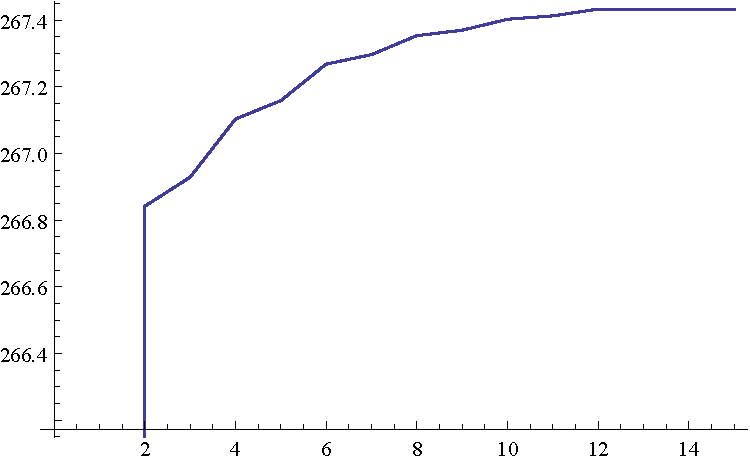
\includegraphics[width=\textwidth]{alphascalarconvground2}
                \caption{Zoom in the flat region}
\end{subfigure}


\caption{Convergence of the polarizability value for the ground state $1s2s_{1/2}$ at 1070 nm.}
\label{alphaconv2}

\end{figure}

\section{Depth of the crossed dipole trap}
\begin{figure}[H]
\centering
 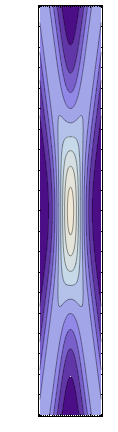
\includegraphics[width=0.2\textwidth,angle=90]{crossed_dipole_trap}

\caption{Schematic intensity distribution for crossed dipole trap. The depth is decided by the maximum intensity in the center, that can be calculated considering a gaussian profile.}
\label{dipolegraphic}
\end{figure}

We now want to calculate the trap depth and the differential light shift, that can be meassured in the experiment. Since the ground state and the first excited states have different polarizabilities, also the light shift is varying. That means, that the energy-difference between the two states changes in case of incoming trap-light and as a result the resonance-frequency of the transition shifts, which can be much easier meassured than the actual depth of the trap. Although the crossed dipole-trap is not a single beam, the beam profile in the middle, where the intensity is at its maximum, is gaussian. That means, that like for a normal gaussian beam, the trap is characterized by its beam-power and waist. The power in this case is two times the power leaving the laser initially, since it gets reflected and forms the second beam as well. The waist in this case is 40 \mu m, with an error estimated to be around 5\%. The experiment will later be performed at multible powers, that have a much higher accuracy with an error, being roughly 0.1\%.
\begin{figure}[h]
\centering
\begin{subfigure}[b]{0.4\textwidth}
                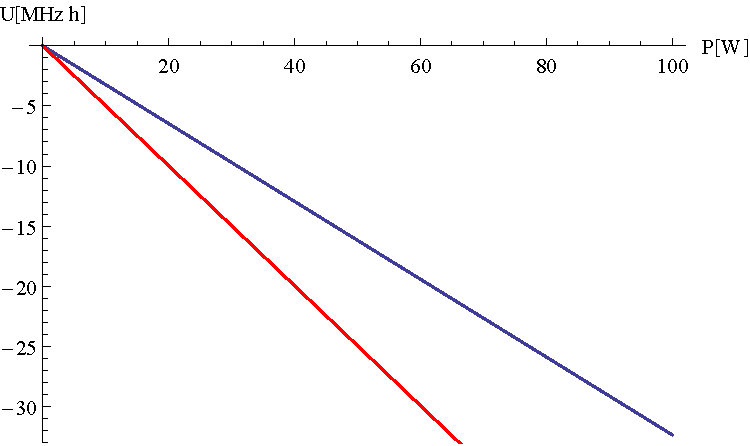
\includegraphics[width=\textwidth]{shift}
                \caption{Trap-depth for ground (red) and excited (blue) state.}
\end{subfigure}
\begin{subfigure}[b]{0.4\textwidth}
               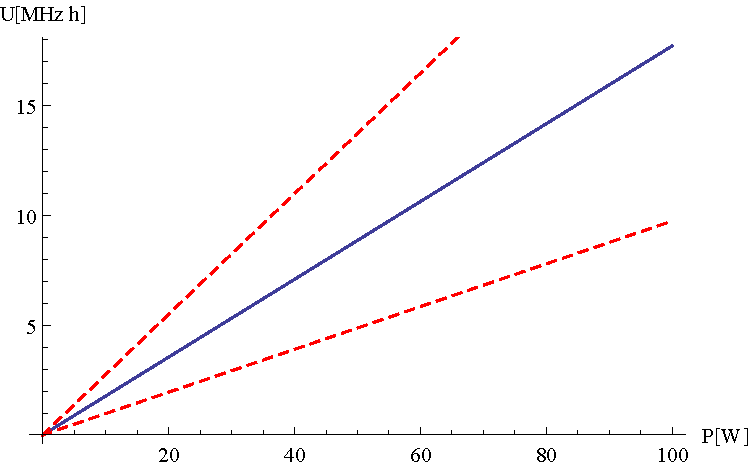
\includegraphics[width=\textwidth]{difshifterror}
                \caption{$D_2$-Resonance-Shift (blue) and the error boundary (red). Slope of $0.175\unit{MHz/W}$}
\end{subfigure}


\caption{Potential for ground ($2s$) and excited ($2p_{3/2}$$|m_J|=3/2$) state and the difference of both, i.e. the shift of the D2-resonance, for different total powers of the trap-beam.}
\label{potential}
\end{figure}
%\begin{figure}[h]
%\begin{center}
%\begin{tabular}{cccc}
%Transition&$\Delta E_\delta [\unit{MHz}\ h]$&$\Delta E_\delta$ at $572\unit{G}  [\unit{MHz }\ h]$&$\Delta\Delta E_\delta [\unit{MHz }\ h]$\\\hline\hline\\
%$2s\rightarrow 2p_{3/2}, |m_j|=1/2$&2.87545&2.87538&1.58106\\
%$2s\rightarrow 2p_{3/2}, |m_j|=3/2$&4.38047&4.38050&1.29365\\
%\\\hline
%\end{tabular}
%\end{center}
%\caption{Differential \textsc{ac}-Stark shift at 50 W of total beam power with and without magnetic field. The sensitivity to the waist-uncertainty leads to a large error and to irrelevance of the magnetic field.}
%\label{relativealpha}
%\end{figure}


\section{Comparison to the classical formula}

Since the classical formula in (\ref{classic}) is widely used to calculate depths for optical dipole traps it is interesting to see, in how far it differs from the quantum-mechanical approach. For the excited state, for allready stated reasons, it is not possible to calculate a good value using this approach, but the ground state, for that the coupling to other states is dominated by the transition to the first excited state, the formula gives values, that differ only 0.3\% when calculating the shift considering transitions up to $n=7$ and using 1070 nm light. When only considering the D-Line transition, both values are the same in range and differ about 0.01 \%. That shows, that using the approach of a harmonic oscillator to model the dipole-trap potential gives good results, when dealing with a system that can be approximated to only consist of two states. In the case of the Lithium-6 ground state, where for infrared light and higher excited states the transitions are very farly detuned, the model gives a good estimate, that is less complicated to calculate than the approach of pertubation theory.
\chapter{Measurements}
For evaluating the calulations in the experiment the resonance-frequency of the D2-Line was measured. 



\section{Evaluation}
\begin{figure}[H]
\centering
\begin{subfigure}[b]{0.48\textwidth}
                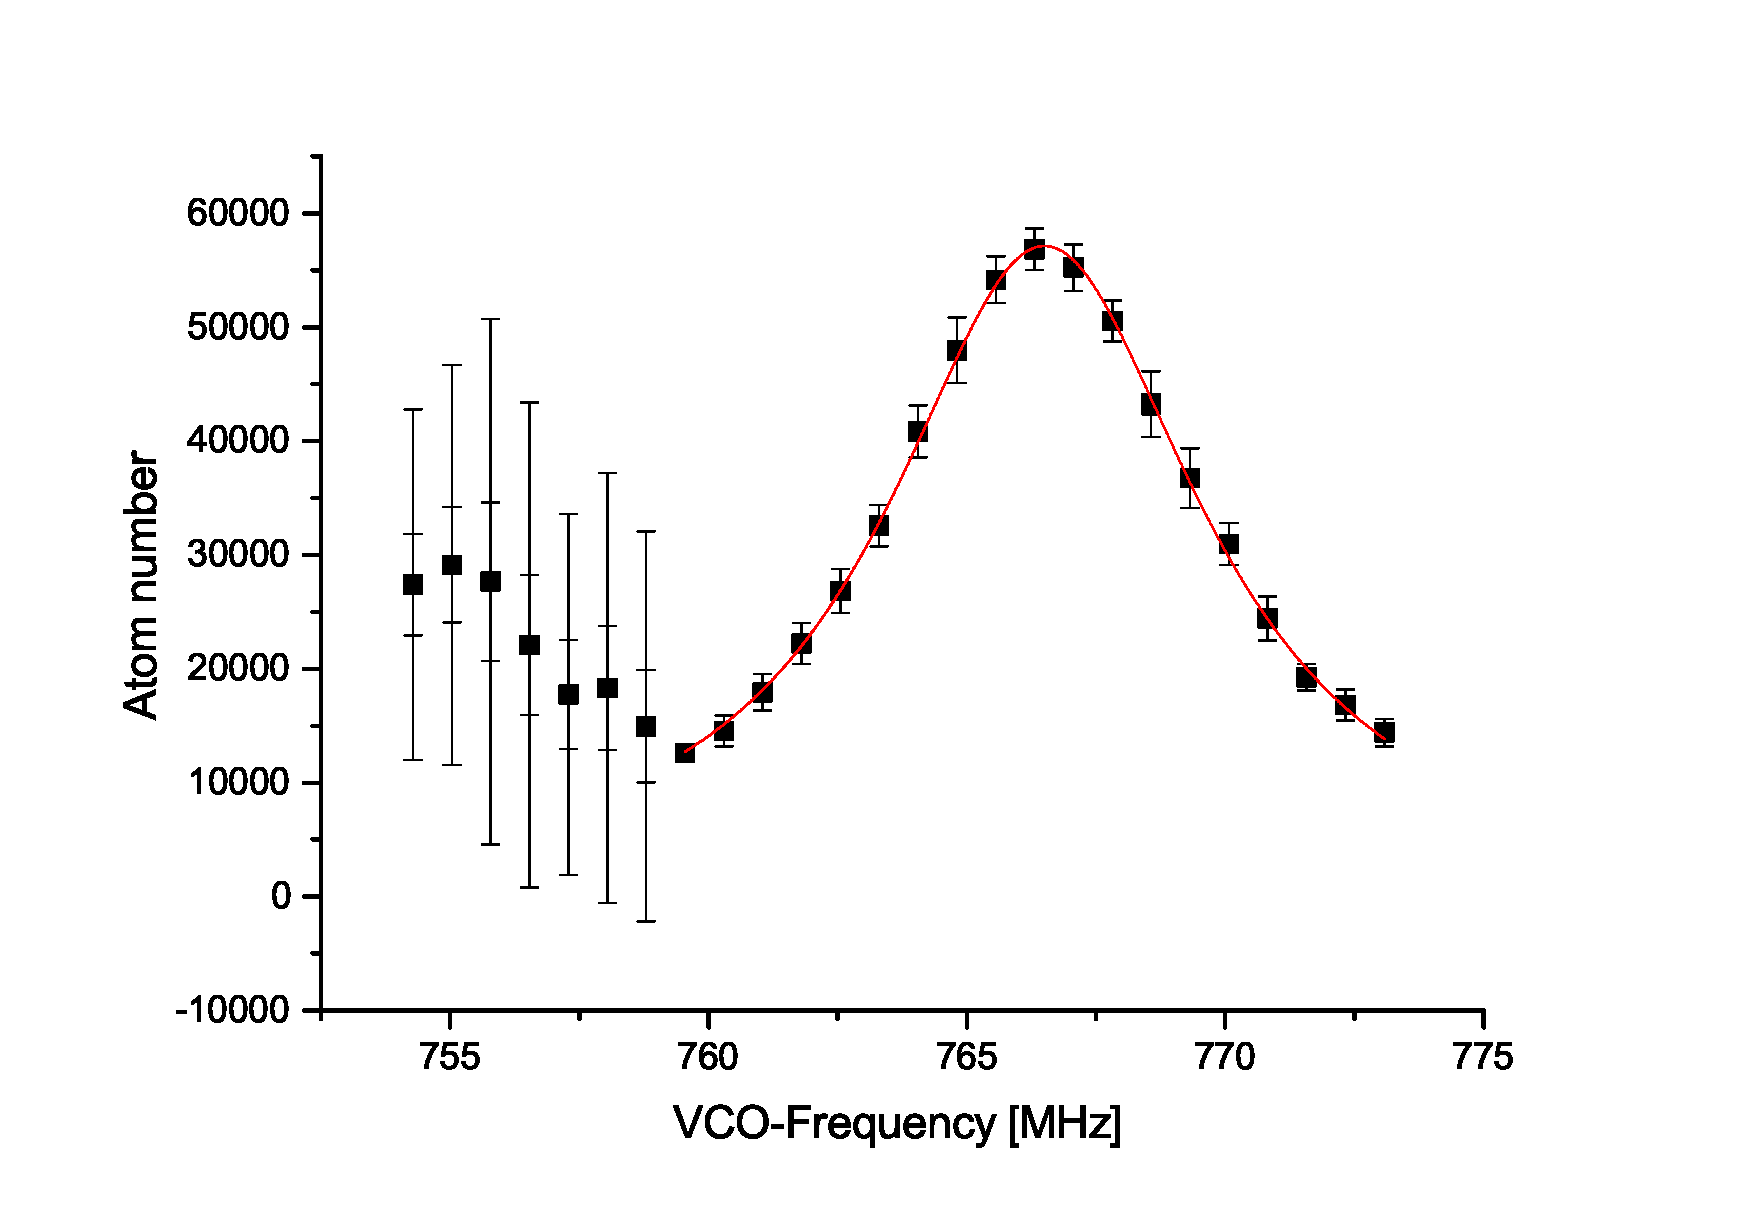
\includegraphics[width=\textwidth]{withoutodt}
                \caption{Dipole-trap turned off.}
\end{subfigure}
\begin{subfigure}[b]{0.48\textwidth}
               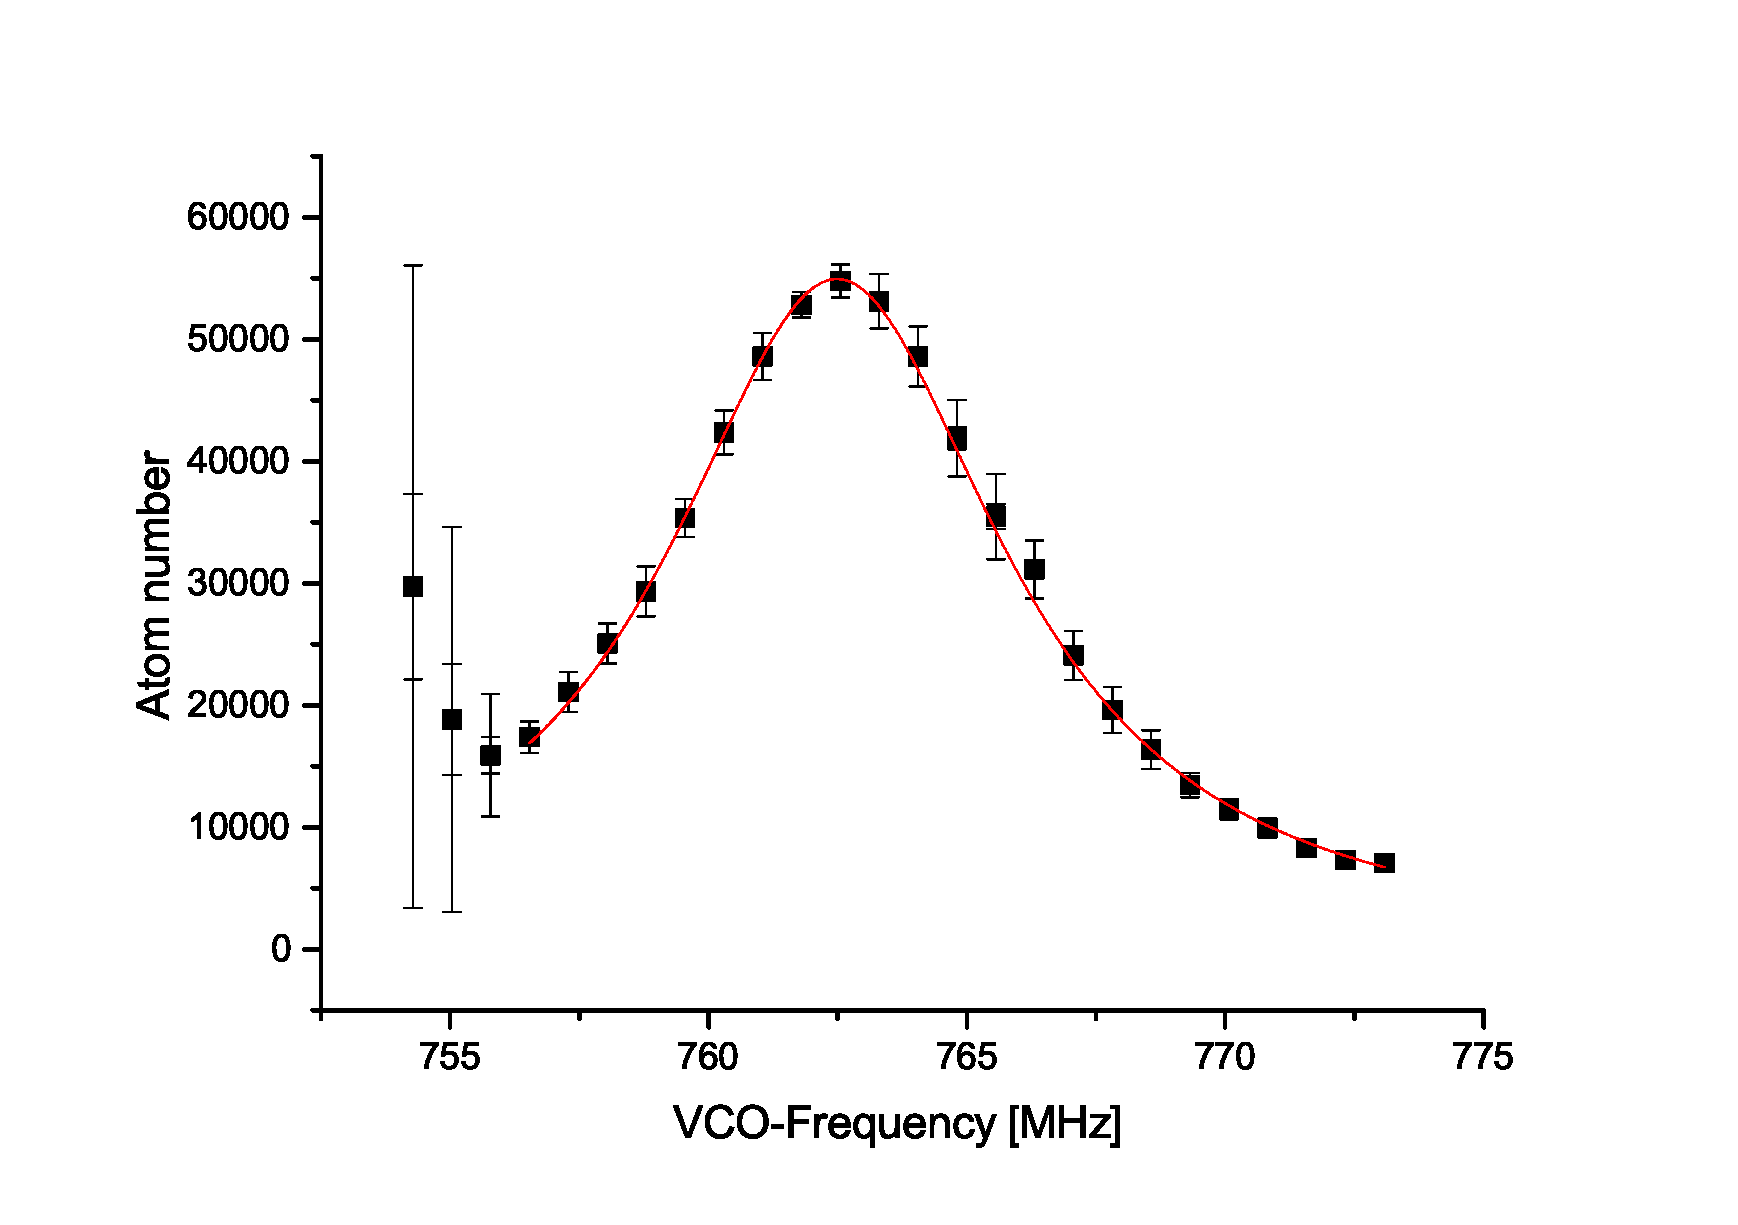
\includegraphics[width=\textwidth]{withodt}
                \caption{Dipole-trap turned on.}
\end{subfigure}


\caption{Resonance peak for the transition: $2s\rightarrow2p_{3/2}, m_j=+3/2$ at 1070 nm. The power at this meassurement was 12.35 W. The scale shows frequencies of the voltrage-controlled oscillator determning the detuning of the laser and is fixed arbitrairily. It therefore shows only the relative shift. A Lorentzian function (red) was fitted to the values, whose parameters were used to determine the center position of the peak. In the range, where the laser was effectivly off-resonance the seen atom-cloud lost its gaussian profile, and therefore no fit was possible to determine the atom number. This accounts for the high errors in this range.}
\label{resonance}
\end{figure}

The measurement of the \textsc{ac}-Stark shift is done in the crossed dipole-trap. For technical reasons the magnetic field was at 527 G for every measurement. As calculated before this should not change the behaviour of the light shift significantly. To find the resonance peak in the respective setting the atom number is meassured using absorbtion imaging. The frequency of the imaging-laser is hereby scanned over the considered resonance, taking an image for every step in detuning. To find the differential light shift, the pictures are taken either with the activated dipole-trap or with the laser-beams turned off, leaving minimum time of flight in order to get significant results. For the imaging the $D_2$-line was used, that corresponds to the transition from  $2s\rightarrow2p_{3/2}$. The imaging laser was $\sigma^+$-polarized. Therefore the excited state was in the magnetic sublevel $m_j=+3/2$. The resonance frequency of this transition is 670.977 nm. Since the excited state is expected to be shifted less strong than the ground state, the energy difference should decrease, leading to a lower resonance frequency and a higher resonance wavelength. The shift is expected to be 0.175\pm 0.060 MHz/W and therefore the resonance frequency for 12.35 W should be 4.3\pm 1.5 MHz lower, when activating the dipoletrap. The resulting graph for this power can be seen in figure \ref{resonance}. To compare the behaviour as well as the exact values with the theory, different powers were measured and plotted in figure \ref{shifts}. 

\begin{figure}[H]
\centering
\begin{subfigure}[b]{0.8\textwidth}
                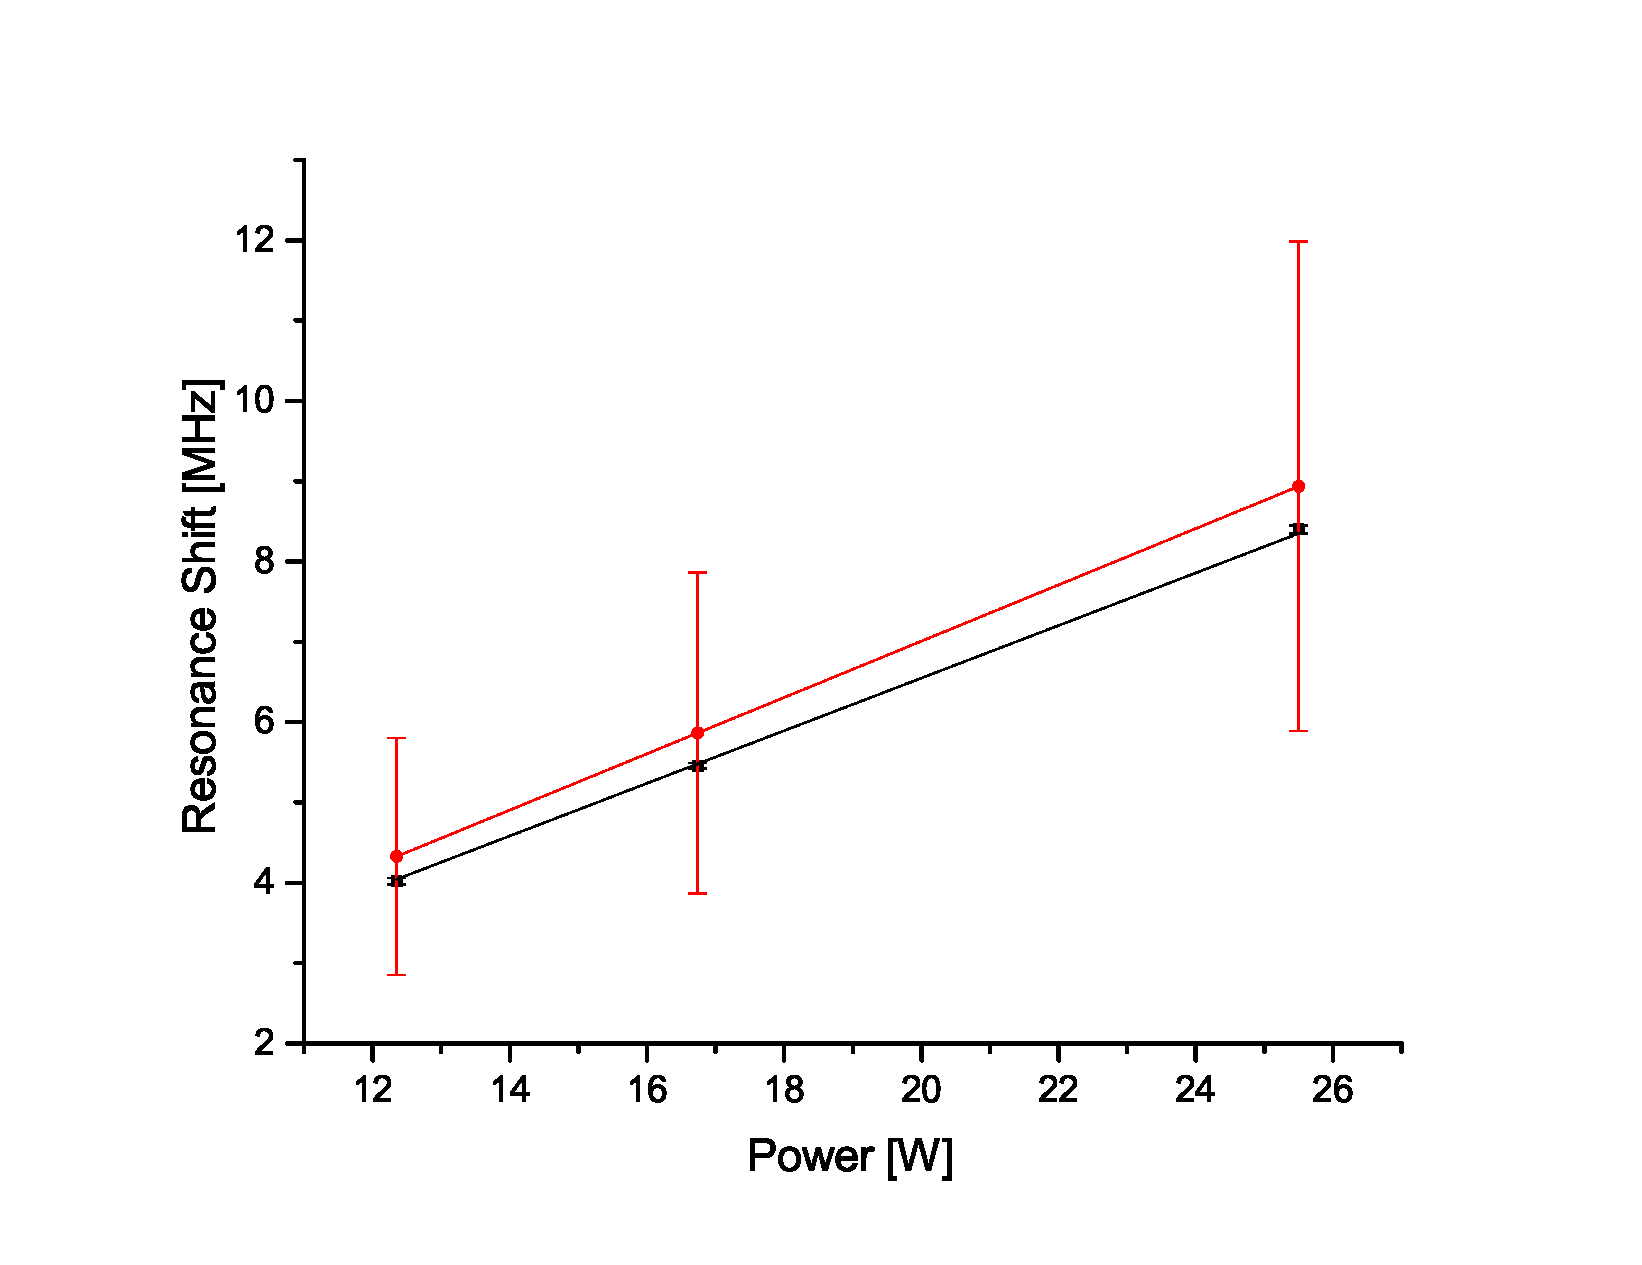
\includegraphics[width=\textwidth]{Shift2}
\end{subfigure}
\caption{Comparison of the differential light-shift in theory (red) and experiment (black) for the D2-line. Note, that the scales show the initial laser-powers. The power in the middle of the trap itself is twice as strong. As is visible in this plot, the errors for the measured shifts are very small compared to that of the calculated value. This supports the assumption, that the error is mostly systematic and can be removed in comparrison with the measured results.}
\label{shifts}
\end{figure}


As can be seen in figure \ref{shifts} the shifts show a linear behaviour. The fit was fixed at ($P=0, \Delta E_\mathrm{dif}=0$) and still shows a very good result. The slope is $0.3274\pm 0.0013\unit{MHz/W}$ of initial beam-power. For a more general statement the value is also given in terms of the intensity:
\begin{figure}[h]
\centering
\begin{subfigure}[b]{0.8\textwidth}
                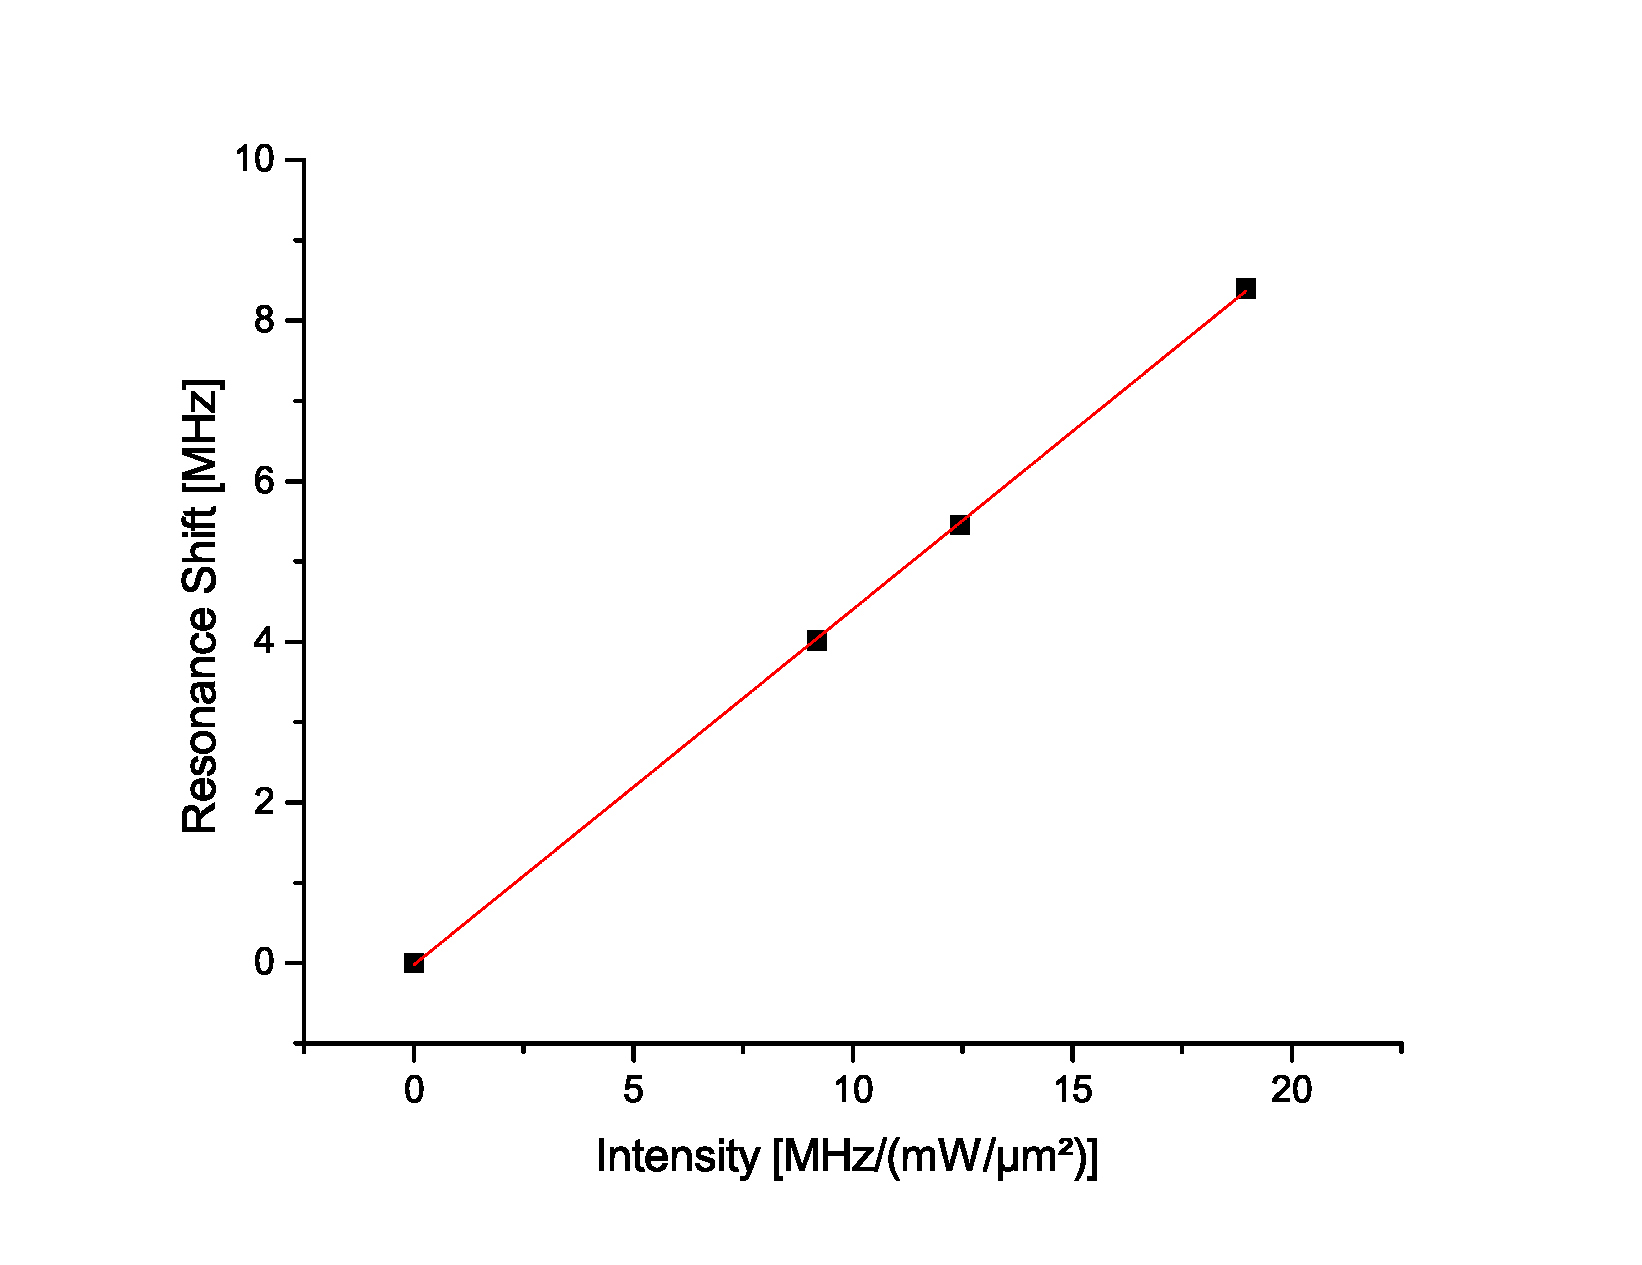
\includegraphics[width=\textwidth]{shiftintens}
\end{subfigure}
\caption{Measured differential shift in terms of intensity.}
\label{shiftintens}
\end{figure}
\begin{equation}
\Delta E_\mathrm{dif}/I=0.4426\pm 0.0028\unit{MHz\frac{1}{mW/\mu m^2}}
\end{equation}
Using this value, we also can calculate the trap depth, when knowing the relation of both polarizabilities for gound and excited states. The formula is derived using the fact, that the relation between the polarizabilities and thus the lightshifts is constant for every power.
\begin{align}
U_{\mathrm{g}}=&-\frac{1}{1-\alpha_{\mathrm{e}}/\alpha_{\mathrm{g}}}\cdot \Delta E_\delta\\
U_{\mathrm{e}}=&-\frac{1}{1-\alpha_{\mathrm{g}}/\alpha_{\mathrm{e}}}\cdot \Delta E_\delta
\end{align}
In this case $\Delta E_\delta$ stands for the relative shift of the levels relative to each other, i.e. the shift of the resonance. The results of the experiment translate into depths of the trap potential for the ground and excited state with the following values:
\begin{align}
U_g/I=&-(120.32\pm 0.48)\unit{\mu K\ k_B\frac{1}{mW/\mu m^2}}\\
U_e/I=&-(78.05\pm 0.31)\unit{\mu K\ k_B\frac{1}{mW/\mu m^2}}
\end{align}
Also the measurement can make it possible to find values for other quantities of the trap. The waist of the trap beam for example is usually not exactly easy to meassure, in contrast to its power, that we know with good precision.
\begin{align}
I=&\frac{\epsilon_0 c}{\alpha}\cdot U\\\notag\\
w_0=&\sqrt{\frac{2P}{\pi I}}
\end{align}
In this calculation $I$ is the actual maximum-intensity forming the potential and $P$ the initial laser-power in the trap. For the crossed dipole-trap this results in the following waist.
\begin{equation}
w_0=41.383\pm 0.082\unit{\mu m}
\end{equation}
The approximate value used for the calculation, taken from \cite{lompe} was 40\mu m.

\subsection{Microtrap parameters}

Trusting the tested theory we now can calculate the depth for the microtrap in that the flourescence imaging is meant to be implemented. The current waist of the trap is 1.3 $\mu$m using laser power of 400 $\mu$\textsc{w}. This leads to a trap depth of
\begin{align}
U_g=&-(6.03\pm 0.61)\unit{\mu K}\ k_B\\
U_e=&-(3.90\pm 0.39)\unit{\mu K}\ k_B
\end{align}
Assuming a 5\%-error on the beams waist. We can use $p_\gamma=h/\lambda$ and $T_{Li}=p^2/2m_{Li}$ to calculate the kinetic energy of an excited Lithium-6 atom. The trap depth corresponts roughly to the momentum of only a single photon, that is reemitted in a random direction. Therefore the trap is not deep enough for holding an atom for enough absorbtion events to actually measure the fluorescence. However, it is possible in our setup to ramp the laserpower up to about 500 mW, that would correspond to the energy of about 1400 photon recoil energies.
\begin{align}
U_g=&-(7.54\pm 0.76)\unit{mK}\ k_B\\
U_e=&-(4.88\pm 0.49)\unit{mK}\ k_B
\end{align}



\printbibliography

\end{document}

